\documentclass[1p]{elsarticle_modified}
%\bibliographystyle{elsarticle-num}

%\usepackage[colorlinks]{hyperref}
%\usepackage{abbrmath_seonhwa} %\Abb, \Ascr, \Acal ,\Abf, \Afrak
\usepackage{amsfonts}
\usepackage{amssymb}
\usepackage{amsmath}
\usepackage{amsthm}
\usepackage{scalefnt}
\usepackage{amsbsy}
\usepackage{kotex}
\usepackage{caption}
\usepackage{subfig}
\usepackage{color}
\usepackage{graphicx}
\usepackage{xcolor} %% white, black, red, green, blue, cyan, magenta, yellow
\usepackage{float}
\usepackage{setspace}
\usepackage{hyperref}

\usepackage{tikz}
\usetikzlibrary{arrows}

\usepackage{multirow}
\usepackage{array} % fixed length table
\usepackage{hhline}

%%%%%%%%%%%%%%%%%%%%%
\makeatletter
\renewcommand*\env@matrix[1][\arraystretch]{%
	\edef\arraystretch{#1}%
	\hskip -\arraycolsep
	\let\@ifnextchar\new@ifnextchar
	\array{*\c@MaxMatrixCols c}}
\makeatother %https://tex.stackexchange.com/questions/14071/how-can-i-increase-the-line-spacing-in-a-matrix
%%%%%%%%%%%%%%%

\usepackage[normalem]{ulem}

\newcommand{\msout}[1]{\ifmmode\text{\sout{\ensuremath{#1}}}\else\sout{#1}\fi}
%SOURCE: \msout is \stkout macro in https://tex.stackexchange.com/questions/20609/strikeout-in-math-mode

\newcommand{\cancel}[1]{
	\ifmmode
	{\color{red}\msout{#1}}
	\else
	{\color{red}\sout{#1}}
	\fi
}

\newcommand{\add}[1]{
	{\color{blue}\uwave{#1}}
}

\newcommand{\replace}[2]{
	\ifmmode
	{\color{red}\msout{#1}}{\color{blue}\uwave{#2}}
	\else
	{\color{red}\sout{#1}}{\color{blue}\uwave{#2}}
	\fi
}

\newcommand{\Sol}{\mathcal{S}} %segment
\newcommand{\D}{D} %diagram
\newcommand{\A}{\mathcal{A}} %arc


%%%%%%%%%%%%%%%%%%%%%%%%%%%%%5 test

\def\sl{\operatorname{\textup{SL}}(2,\Cbb)}
\def\psl{\operatorname{\textup{PSL}}(2,\Cbb)}
\def\quan{\mkern 1mu \triangleright \mkern 1mu}

\theoremstyle{definition}
\newtheorem{thm}{Theorem}[section]
\newtheorem{prop}[thm]{Proposition}
\newtheorem{lem}[thm]{Lemma}
\newtheorem{ques}[thm]{Question}
\newtheorem{cor}[thm]{Corollary}
\newtheorem{defn}[thm]{Definition}
\newtheorem{exam}[thm]{Example}
\newtheorem{rmk}[thm]{Remark}
\newtheorem{alg}[thm]{Algorithm}

\newcommand{\I}{\sqrt{-1}}
\begin{document}

%\begin{frontmatter}
%
%\title{Boundary parabolic representations of knots up to 8 crossings}
%
%%% Group authors per affiliation:
%\author{Yunhi Cho} 
%\address{Department of Mathematics, University of Seoul, Seoul, Korea}
%\ead{yhcho@uos.ac.kr}
%
%
%\author{Seonhwa Kim} %\fnref{s_kim}}
%\address{Center for Geometry and Physics, Institute for Basic Science, Pohang, 37673, Korea}
%\ead{ryeona17@ibs.re.kr}
%
%\author{Hyuk Kim}
%\address{Department of Mathematical Sciences, Seoul National University, Seoul 08826, Korea}
%\ead{hyukkim@snu.ac.kr}
%
%\author{Seokbeom Yoon}
%\address{Department of Mathematical Sciences, Seoul National University, Seoul, 08826,  Korea}
%\ead{sbyoon15@snu.ac.kr}
%
%\begin{abstract}
%We find all boundary parabolic representation of knots up to 8 crossings.
%
%\end{abstract}
%\begin{keyword}
%    \MSC[2010] 57M25 
%\end{keyword}
%
%\end{frontmatter}

%\linenumbers
%\tableofcontents
%
\newcommand\colored[1]{\textcolor{white}{\rule[-0.35ex]{0.8em}{1.4ex}}\kern-0.8em\color{red} #1}%
%\newcommand\colored[1]{\textcolor{white}{ #1}\kern-2.17ex	\textcolor{white}{ #1}\kern-1.81ex	\textcolor{white}{ #1}\kern-2.15ex\color{red}#1	}

{\Large $\underline{12a_{0990}~(K12a_{0990})}$}

\setlength{\tabcolsep}{10pt}
\renewcommand{\arraystretch}{1.6}
\vspace{1cm}\begin{tabular}{m{100pt}>{\centering\arraybackslash}m{274pt}}
\multirow{5}{120pt}{
	\centering
	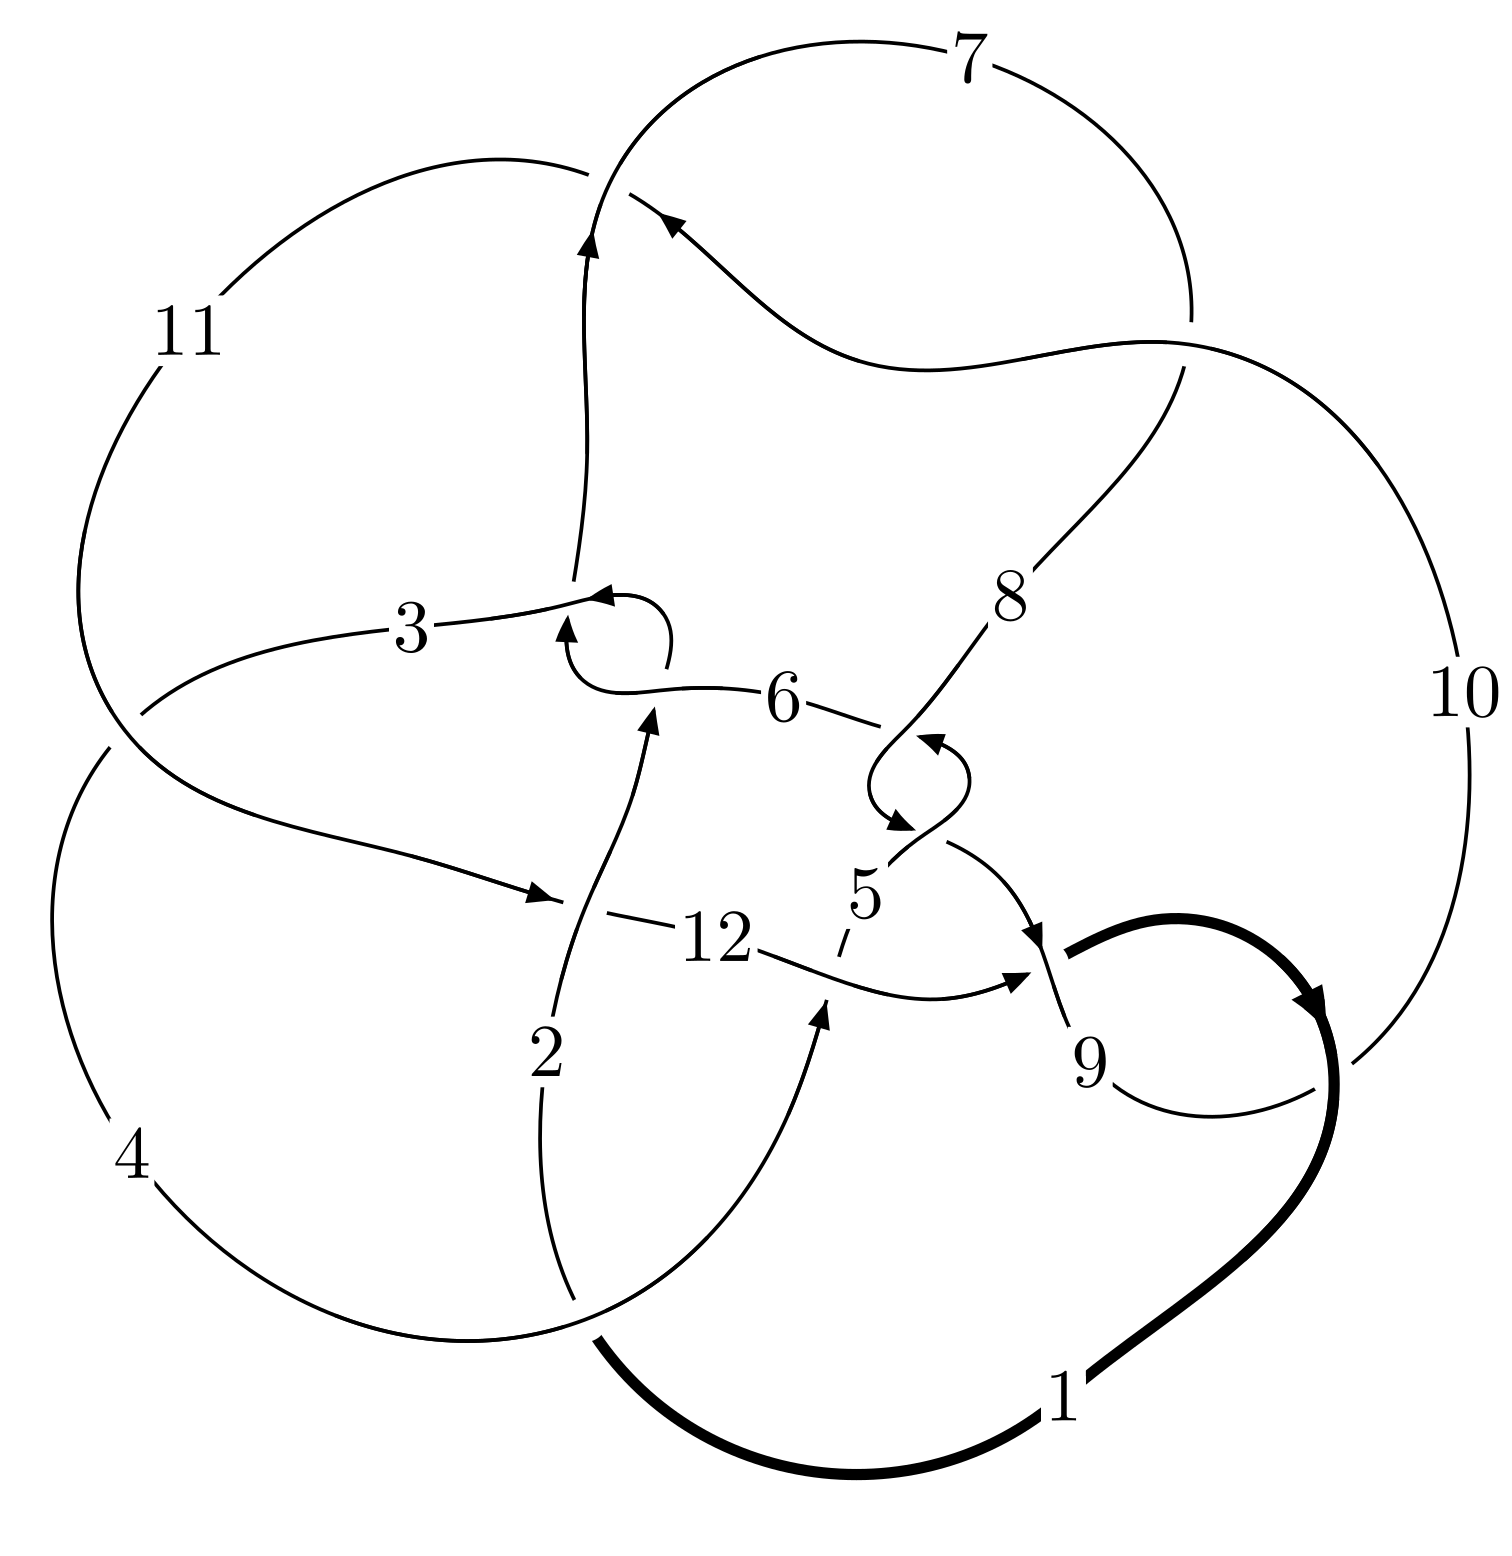
\includegraphics[width=112pt]{../../../GIT/diagram.site/Diagrams/png/1791_12a_0990.png}\\
\ \ \ A knot diagram\footnotemark}&
\allowdisplaybreaks
\textbf{Linearized knot diagam} \\
\cline{2-2}
 &
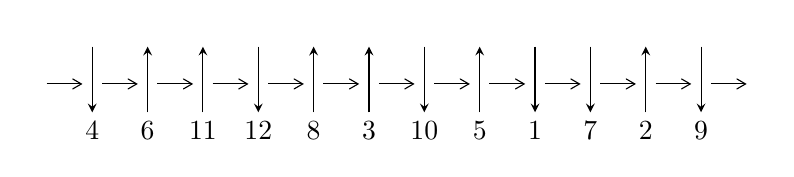
\begin{tikzpicture}[x=20pt, y=17pt]
	% nodes
	\node (C0) at (0, 0) {};
	\node (C1) at (1, 0) {};
	\node (C1U) at (1, +1) {};
	\node (C1D) at (1, -1) {4};

	\node (C2) at (2, 0) {};
	\node (C2U) at (2, +1) {};
	\node (C2D) at (2, -1) {6};

	\node (C3) at (3, 0) {};
	\node (C3U) at (3, +1) {};
	\node (C3D) at (3, -1) {11};

	\node (C4) at (4, 0) {};
	\node (C4U) at (4, +1) {};
	\node (C4D) at (4, -1) {12};

	\node (C5) at (5, 0) {};
	\node (C5U) at (5, +1) {};
	\node (C5D) at (5, -1) {8};

	\node (C6) at (6, 0) {};
	\node (C6U) at (6, +1) {};
	\node (C6D) at (6, -1) {3};

	\node (C7) at (7, 0) {};
	\node (C7U) at (7, +1) {};
	\node (C7D) at (7, -1) {10};

	\node (C8) at (8, 0) {};
	\node (C8U) at (8, +1) {};
	\node (C8D) at (8, -1) {5};

	\node (C9) at (9, 0) {};
	\node (C9U) at (9, +1) {};
	\node (C9D) at (9, -1) {1};

	\node (C10) at (10, 0) {};
	\node (C10U) at (10, +1) {};
	\node (C10D) at (10, -1) {7};

	\node (C11) at (11, 0) {};
	\node (C11U) at (11, +1) {};
	\node (C11D) at (11, -1) {2};

	\node (C12) at (12, 0) {};
	\node (C12U) at (12, +1) {};
	\node (C12D) at (12, -1) {9};
	\node (C13) at (13, 0) {};

	% arrows
	\draw[->,>={angle 60}]
	(C0) edge (C1) (C1) edge (C2) (C2) edge (C3) (C3) edge (C4) (C4) edge (C5) (C5) edge (C6) (C6) edge (C7) (C7) edge (C8) (C8) edge (C9) (C9) edge (C10) (C10) edge (C11) (C11) edge (C12) (C12) edge (C13) ;	\draw[->,>=stealth]
	(C1U) edge (C1D) (C2D) edge (C2U) (C3D) edge (C3U) (C4U) edge (C4D) (C5D) edge (C5U) (C6D) edge (C6U) (C7U) edge (C7D) (C8D) edge (C8U) (C9U) edge (C9D) (C10U) edge (C10D) (C11D) edge (C11U) (C12U) edge (C12D) ;
	\end{tikzpicture} \\
\hhline{~~} \\& 
\textbf{Solving Sequence} \\ \cline{2-2} 
 &
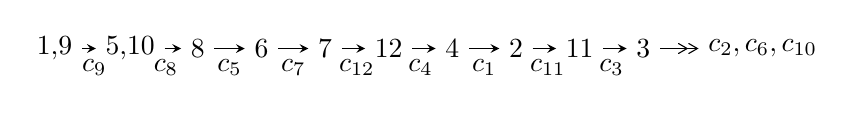
\begin{tikzpicture}[x=23pt, y=7pt]
	% node
	\node (A0) at (-1/8, 0) {1,9};
	\node (A1) at (17/16, 0) {5,10};
	\node (A2) at (17/8, 0) {8};
	\node (A3) at (25/8, 0) {6};
	\node (A4) at (33/8, 0) {7};
	\node (A5) at (41/8, 0) {12};
	\node (A6) at (49/8, 0) {4};
	\node (A7) at (57/8, 0) {2};
	\node (A8) at (65/8, 0) {11};
	\node (A9) at (73/8, 0) {3};
	\node (C1) at (1/2, -1) {$c_{9}$};
	\node (C2) at (13/8, -1) {$c_{8}$};
	\node (C3) at (21/8, -1) {$c_{5}$};
	\node (C4) at (29/8, -1) {$c_{7}$};
	\node (C5) at (37/8, -1) {$c_{12}$};
	\node (C6) at (45/8, -1) {$c_{4}$};
	\node (C7) at (53/8, -1) {$c_{1}$};
	\node (C8) at (61/8, -1) {$c_{11}$};
	\node (C9) at (69/8, -1) {$c_{3}$};
	\node (A10) at (11, 0) {$c_{2},c_{6},c_{10}$};

	% edge
	\draw[->,>=stealth]	
	(A0) edge (A1) (A1) edge (A2) (A2) edge (A3) (A3) edge (A4) (A4) edge (A5) (A5) edge (A6) (A6) edge (A7) (A7) edge (A8) (A8) edge (A9) ;
	\draw[->>,>={angle 60}]	
	(A9) edge (A10);
\end{tikzpicture} \\ 

\end{tabular} \\

\footnotetext{
The image of knot diagram is generated by the software ``\textbf{Draw programme}" developed by Andrew Bartholomew(\url{http://www.layer8.co.uk/maths/draw/index.htm\#Running-draw}), where we modified some parts for our purpose(\url{https://github.com/CATsTAILs/LinksPainter}).
}\phantom \\ \newline 
\centering \textbf{Ideals for irreducible components\footnotemark of $X_{\text{par}}$} 
 
\begin{align*}
I^u_{1}&=\langle 
-7.42364\times10^{545} u^{129}-6.71560\times10^{546} u^{128}+\cdots+2.82169\times10^{548} b-2.11413\times10^{552},\\
\phantom{I^u_{1}}&\phantom{= \langle  }-1.02551\times10^{550} u^{129}-9.21321\times10^{550} u^{128}+\cdots+1.46192\times10^{552} a-2.73974\times10^{556},\\
\phantom{I^u_{1}}&\phantom{= \langle  }u^{130}+10 u^{129}+\cdots+40002776 u+2811556\rangle \\
I^u_{2}&=\langle 
-8.19734\times10^{33} u^{31}-4.22264\times10^{34} u^{30}+\cdots+9.32464\times10^{31} b-8.66565\times10^{34},\\
\phantom{I^u_{2}}&\phantom{= \langle  }-1.09826\times10^{34} u^{31}-5.65664\times10^{34} u^{30}+\cdots+9.32464\times10^{31} a-1.17253\times10^{35},\\
\phantom{I^u_{2}}&\phantom{= \langle  }u^{32}+6 u^{31}+\cdots+48 u+9\rangle \\
I^u_{3}&=\langle 
-9 a^4-16 a^3-76 a^2+13 b-40 a-8,\;a^5+2 a^4+9 a^3+6 a^2+3 a+1,\;u-1\rangle \\
I^u_{4}&=\langle 
b^5-2 b^4 a+b^3 a^2- b^3+a^2 b+b+a-1,\;u-1\rangle \\
\\
I^v_{1}&=\langle 
a,\;b^5+b^3+b+1,\;v-1\rangle \\
I^v_{2}&=\langle 
a,\;b^2- b+1,\;v-1\rangle \\
\end{align*}
\raggedright * 5 irreducible components of $\dim_{\mathbb{C}}=0$, with total 174 representations.\\
\raggedright * 1 irreducible components of $\dim_{\mathbb{C}}=1$ \\
\footnotetext{All coefficients of polynomials are rational numbers. But the coefficients are sometimes approximated in decimal forms when there is not enough margin.}
\newpage
\renewcommand{\arraystretch}{1}
\centering \section*{I. $I^u_{1}= \langle -7.42\times10^{545} u^{129}-6.72\times10^{546} u^{128}+\cdots+2.82\times10^{548} b-2.11\times10^{552},\;-1.03\times10^{550} u^{129}-9.21\times10^{550} u^{128}+\cdots+1.46\times10^{552} a-2.74\times10^{556},\;u^{130}+10 u^{129}+\cdots+40002776 u+2811556 \rangle$}
\flushleft \textbf{(i) Arc colorings}\\
\begin{tabular}{m{7pt} m{180pt} m{7pt} m{180pt} }
\flushright $a_{1}=$&$\begin{pmatrix}0\\u\end{pmatrix}$ \\
\flushright $a_{9}=$&$\begin{pmatrix}1\\0\end{pmatrix}$ \\
\flushright $a_{5}=$&$\begin{pmatrix}0.00701480 u^{129}+0.0630213 u^{128}+\cdots+249589. u+18740.7\\0.00263092 u^{129}+0.0237999 u^{128}+\cdots+99398.1 u+7492.40\end{pmatrix}$ \\
\flushright $a_{10}=$&$\begin{pmatrix}1\\u^2\end{pmatrix}$ \\
\flushright $a_{8}=$&$\begin{pmatrix}0.00101759 u^{129}+0.00900101 u^{128}+\cdots+33569.9 u+2537.03\\0.000471567 u^{129}+0.00411483 u^{128}+\cdots+11762.5 u+842.151\end{pmatrix}$ \\
\flushright $a_{6}=$&$\begin{pmatrix}0.00126397 u^{129}+0.0107887 u^{128}+\cdots+28928.9 u+2098.07\\-0.000934236 u^{129}-0.00863981 u^{128}+\cdots-40675.0 u-3104.76\end{pmatrix}$ \\
\flushright $a_{7}=$&$\begin{pmatrix}0.000150095 u^{129}+0.00122081 u^{128}+\cdots+1195.24 u+75.9623\\-0.000473077 u^{129}-0.00432755 u^{128}+\cdots-21590.6 u-1673.46\end{pmatrix}$ \\
\flushright $a_{12}=$&$\begin{pmatrix}u\\u\end{pmatrix}$ \\
\flushright $a_{4}=$&$\begin{pmatrix}0.00233873 u^{129}+0.0208067 u^{128}+\cdots+77208.8 u+5758.85\\-0.00204515 u^{129}-0.0184147 u^{128}+\cdots-72982.4 u-5489.48\end{pmatrix}$ \\
\flushright $a_{2}=$&$\begin{pmatrix}0.000274293 u^{129}+0.00247203 u^{128}+\cdots+11517.0 u+900.409\\0.000908201 u^{129}+0.00823727 u^{128}+\cdots+35139.9 u+2659.78\end{pmatrix}$ \\
\flushright $a_{11}=$&$\begin{pmatrix}0.000756422 u^{129}+0.00676781 u^{128}+\cdots+27485.4 u+2094.49\\-0.000620407 u^{129}-0.00564869 u^{128}+\cdots-24415.3 u-1859.15\end{pmatrix}$ \\
\flushright $a_{3}=$&$\begin{pmatrix}-0.00217529 u^{129}-0.0186835 u^{128}+\cdots-48388.1 u-3437.17\\-0.000312213 u^{129}-0.00218499 u^{128}+\cdots+8773.04 u+748.786\end{pmatrix}$\\&\end{tabular}
\flushleft \textbf{(ii) Obstruction class $= -1$}\\~\\
\flushleft \textbf{(iii) Cusp Shapes $= -0.00272619 u^{129}-0.0236021 u^{128}+\cdots-76099.3 u-5729.03$}\\~\\
\newpage\renewcommand{\arraystretch}{1}
\flushleft \textbf{(iv) u-Polynomials at the component}\newline \\
\begin{tabular}{m{50pt}|m{274pt}}
Crossings & \hspace{64pt}u-Polynomials at each crossing \\
\hline $$\begin{aligned}c_{1}\end{aligned}$$&$\begin{aligned}
&16(16 u^{130}-216 u^{129}+\cdots-134148 u+11877)
\end{aligned}$\\
\hline $$\begin{aligned}c_{2},c_{6}\end{aligned}$$&$\begin{aligned}
&u^{130}+10 u^{129}+\cdots+40002776 u+2811556
\end{aligned}$\\
\hline $$\begin{aligned}c_{3}\end{aligned}$$&$\begin{aligned}
&48(48 u^{130}-144 u^{129}+\cdots-1.54523\times10^{9} u+4.56957\times10^{8})
\end{aligned}$\\
\hline $$\begin{aligned}c_{4}\end{aligned}$$&$\begin{aligned}
&48(48 u^{130}+144 u^{129}+\cdots+1.54523\times10^{9} u+4.56957\times10^{8})
\end{aligned}$\\
\hline $$\begin{aligned}c_{5},c_{8}\end{aligned}$$&$\begin{aligned}
&16(16 u^{130}+72 u^{129}+\cdots+6.78136\times10^{7} u+7939137)
\end{aligned}$\\
\hline $$\begin{aligned}c_{7},c_{10}\end{aligned}$$&$\begin{aligned}
&16(16 u^{130}-72 u^{129}+\cdots-6.78136\times10^{7} u+7939137)
\end{aligned}$\\
\hline $$\begin{aligned}c_{9},c_{12}\end{aligned}$$&$\begin{aligned}
&u^{130}-10 u^{129}+\cdots-40002776 u+2811556
\end{aligned}$\\
\hline $$\begin{aligned}c_{11}\end{aligned}$$&$\begin{aligned}
&16(16 u^{130}+216 u^{129}+\cdots+134148 u+11877)
\end{aligned}$\\
\hline
\end{tabular}\\~\\
\newpage\renewcommand{\arraystretch}{1}
\flushleft \textbf{(v) Riley Polynomials at the component}\newline \\
\begin{tabular}{m{50pt}|m{274pt}}
Crossings & \hspace{64pt}Riley Polynomials at each crossing \\
\hline $$\begin{aligned}c_{1},c_{11}\end{aligned}$$&$\begin{aligned}
&256(256 y^{130}-4640 y^{129}+\cdots+2.95033\times10^{9} y+1.41063\times10^{8})
\end{aligned}$\\
\hline $$\begin{aligned}c_{2},c_{6},c_{9}\\c_{12}\end{aligned}$$&$\begin{aligned}
&y^{130}-80 y^{129}+\cdots-226520781477232 y+7904847141136
\end{aligned}$\\
\hline $$\begin{aligned}c_{3},c_{4}\end{aligned}$$&$\begin{aligned}
&2304(2304 y^{130}-123744 y^{129}+\cdots-5.35364\times10^{18} y+2.08809\times10^{17})
\end{aligned}$\\
\hline $$\begin{aligned}c_{5},c_{7},c_{8}\\c_{10}\end{aligned}$$&$\begin{aligned}
&256\\
&\cdot(256 y^{130}+23008 y^{129}+\cdots-581798760447684 y+63029896304769)
\end{aligned}$\\
\hline
\end{tabular}\\~\\
\newpage\flushleft \textbf{(vi) Complex Volumes and Cusp Shapes}
$$\begin{array}{c|c|c}  
\text{Solutions to }I^u_{1}& \I (\text{vol} + \sqrt{-1}CS) & \text{Cusp shape}\\
 \hline 
\begin{aligned}
u &= -0.753714 + 0.678165 I \\
a &= -0.429062 - 0.743953 I \\
b &= -0.617531 + 0.243011 I\end{aligned}
 & \phantom{-}2.79527 + 2.32555 I & \phantom{-0.000000 } 0 \\ \hline\begin{aligned}
u &= -0.753714 - 0.678165 I \\
a &= -0.429062 + 0.743953 I \\
b &= -0.617531 - 0.243011 I\end{aligned}
 & \phantom{-}2.79527 - 2.32555 I & \phantom{-0.000000 } 0 \\ \hline\begin{aligned}
u &= \phantom{-}0.364736 + 0.913386 I \\
a &= \phantom{-}0.024867 - 1.138090 I \\
b &= \phantom{-}0.568641 - 0.599752 I\end{aligned}
 & \phantom{-}7.79727 - 3.48496 I & \phantom{-0.000000 } 0 \\ \hline\begin{aligned}
u &= \phantom{-}0.364736 - 0.913386 I \\
a &= \phantom{-}0.024867 + 1.138090 I \\
b &= \phantom{-}0.568641 + 0.599752 I\end{aligned}
 & \phantom{-}7.79727 + 3.48496 I & \phantom{-0.000000 } 0 \\ \hline\begin{aligned}
u &= -0.836988 + 0.515749 I \\
a &= \phantom{-}0.170742 - 0.519532 I \\
b &= -0.865889 - 0.510137 I\end{aligned}
 & \phantom{-}2.40493 + 2.37289 I & \phantom{-0.000000 } 0 \\ \hline\begin{aligned}
u &= -0.836988 - 0.515749 I \\
a &= \phantom{-}0.170742 + 0.519532 I \\
b &= -0.865889 + 0.510137 I\end{aligned}
 & \phantom{-}2.40493 - 2.37289 I & \phantom{-0.000000 } 0 \\ \hline\begin{aligned}
u &= \phantom{-}0.023345 + 1.032480 I \\
a &= \phantom{-}0.370646 + 0.393498 I \\
b &= -0.226301 + 1.308480 I\end{aligned}
 & -1.03079 - 7.20926 I & \phantom{-0.000000 } 0 \\ \hline\begin{aligned}
u &= \phantom{-}0.023345 - 1.032480 I \\
a &= \phantom{-}0.370646 - 0.393498 I \\
b &= -0.226301 - 1.308480 I\end{aligned}
 & -1.03079 + 7.20926 I & \phantom{-0.000000 } 0 \\ \hline\begin{aligned}
u &= -0.014661 + 0.956748 I \\
a &= -0.016413 + 0.251138 I \\
b &= -0.346796 + 1.202210 I\end{aligned}
 & -1.34210 - 3.05609 I & \phantom{-0.000000 } 0 \\ \hline\begin{aligned}
u &= -0.014661 - 0.956748 I \\
a &= -0.016413 - 0.251138 I \\
b &= -0.346796 - 1.202210 I\end{aligned}
 & -1.34210 + 3.05609 I & \phantom{-0.000000 } 0\\
 \hline 
 \end{array}$$\newpage$$\begin{array}{c|c|c}  
\text{Solutions to }I^u_{1}& \I (\text{vol} + \sqrt{-1}CS) & \text{Cusp shape}\\
 \hline 
\begin{aligned}
u &= -1.035250 + 0.190731 I \\
a &= \phantom{-}0.19971 + 3.07796 I \\
b &= \phantom{-}0.320853 + 1.071130 I\end{aligned}
 & \phantom{-}4.01258 + 10.32040 I & \phantom{-0.000000 } 0 \\ \hline\begin{aligned}
u &= -1.035250 - 0.190731 I \\
a &= \phantom{-}0.19971 - 3.07796 I \\
b &= \phantom{-}0.320853 - 1.071130 I\end{aligned}
 & \phantom{-}4.01258 - 10.32040 I & \phantom{-0.000000 } 0 \\ \hline\begin{aligned}
u &= -1.035300 + 0.209769 I \\
a &= -0.09804 - 2.67630 I \\
b &= -0.222571 - 1.175360 I\end{aligned}
 & -0.16136 + 5.32813 I & \phantom{-0.000000 } 0 \\ \hline\begin{aligned}
u &= -1.035300 - 0.209769 I \\
a &= -0.09804 + 2.67630 I \\
b &= -0.222571 + 1.175360 I\end{aligned}
 & -0.16136 - 5.32813 I & \phantom{-0.000000 } 0 \\ \hline\begin{aligned}
u &= \phantom{-}0.934913 + 0.047377 I \\
a &= -1.05680 + 1.64472 I \\
b &= -1.37976 + 0.66931 I\end{aligned}
 & -1.085330 - 0.334255 I & \phantom{-0.000000 } 0 \\ \hline\begin{aligned}
u &= \phantom{-}0.934913 - 0.047377 I \\
a &= -1.05680 - 1.64472 I \\
b &= -1.37976 - 0.66931 I\end{aligned}
 & -1.085330 + 0.334255 I & \phantom{-0.000000 } 0 \\ \hline\begin{aligned}
u &= \phantom{-}0.049853 + 0.924522 I \\
a &= -0.153356 - 0.036650 I \\
b &= \phantom{-}0.542235 - 1.129970 I\end{aligned}
 & \phantom{-}0.16136 - 5.32813 I & \phantom{-0.000000 } 0 \\ \hline\begin{aligned}
u &= \phantom{-}0.049853 - 0.924522 I \\
a &= -0.153356 + 0.036650 I \\
b &= \phantom{-}0.542235 + 1.129970 I\end{aligned}
 & \phantom{-}0.16136 + 5.32813 I & \phantom{-0.000000 } 0 \\ \hline\begin{aligned}
u &= -0.872987 + 0.633017 I \\
a &= \phantom{-}0.805377 + 0.601460 I \\
b &= \phantom{-}0.607331 - 0.671357 I\end{aligned}
 & \phantom{-}5.31312 + 6.77397 I & \phantom{-0.000000 } 0 \\ \hline\begin{aligned}
u &= -0.872987 - 0.633017 I \\
a &= \phantom{-}0.805377 - 0.601460 I \\
b &= \phantom{-}0.607331 + 0.671357 I\end{aligned}
 & \phantom{-}5.31312 - 6.77397 I & \phantom{-0.000000 } 0\\
 \hline 
 \end{array}$$\newpage$$\begin{array}{c|c|c}  
\text{Solutions to }I^u_{1}& \I (\text{vol} + \sqrt{-1}CS) & \text{Cusp shape}\\
 \hline 
\begin{aligned}
u &= -1.072770 + 0.123948 I \\
a &= -0.949991 + 0.241825 I \\
b &= -1.55098 + 0.35434 I\end{aligned}
 & -0.175289 + 0.755522 I & \phantom{-0.000000 } 0 \\ \hline\begin{aligned}
u &= -1.072770 - 0.123948 I \\
a &= -0.949991 - 0.241825 I \\
b &= -1.55098 - 0.35434 I\end{aligned}
 & -0.175289 - 0.755522 I & \phantom{-0.000000 } 0 \\ \hline\begin{aligned}
u &= -0.494026 + 0.973656 I \\
a &= -0.039642 + 0.660869 I \\
b &= \phantom{-}0.549748 + 0.349714 I\end{aligned}
 & \phantom{-}8.28948 - 0.12430 I & \phantom{-0.000000 } 0 \\ \hline\begin{aligned}
u &= -0.494026 - 0.973656 I \\
a &= -0.039642 - 0.660869 I \\
b &= \phantom{-}0.549748 - 0.349714 I\end{aligned}
 & \phantom{-}8.28948 + 0.12430 I & \phantom{-0.000000 } 0 \\ \hline\begin{aligned}
u &= -1.075040 + 0.250971 I \\
a &= \phantom{-}0.44267 + 2.18430 I \\
b &= \phantom{-}0.004035 + 1.026040 I\end{aligned}
 & \phantom{-}3.31794 + 0.02095 I & \phantom{-0.000000 } 0 \\ \hline\begin{aligned}
u &= -1.075040 - 0.250971 I \\
a &= \phantom{-}0.44267 - 2.18430 I \\
b &= \phantom{-}0.004035 - 1.026040 I\end{aligned}
 & \phantom{-}3.31794 - 0.02095 I & \phantom{-0.000000 } 0 \\ \hline\begin{aligned}
u &= \phantom{-}0.456734 + 0.758309 I \\
a &= -0.220146 + 1.329500 I \\
b &= -0.630414 + 0.185361 I\end{aligned}
 & \phantom{-}3.18794 + 2.74835 I & \phantom{-0.000000 } 0 \\ \hline\begin{aligned}
u &= \phantom{-}0.456734 - 0.758309 I \\
a &= -0.220146 - 1.329500 I \\
b &= -0.630414 - 0.185361 I\end{aligned}
 & \phantom{-}3.18794 - 2.74835 I & \phantom{-0.000000 } 0 \\ \hline\begin{aligned}
u &= \phantom{-}0.057062 + 1.121730 I \\
a &= -0.328075 - 0.357135 I \\
b &= \phantom{-}0.081204 - 1.173900 I\end{aligned}
 & -3.18794 - 2.74835 I & \phantom{-0.000000 } 0 \\ \hline\begin{aligned}
u &= \phantom{-}0.057062 - 1.121730 I \\
a &= -0.328075 + 0.357135 I \\
b &= \phantom{-}0.081204 + 1.173900 I\end{aligned}
 & -3.18794 + 2.74835 I & \phantom{-0.000000 } 0\\
 \hline 
 \end{array}$$\newpage$$\begin{array}{c|c|c}  
\text{Solutions to }I^u_{1}& \I (\text{vol} + \sqrt{-1}CS) & \text{Cusp shape}\\
 \hline 
\begin{aligned}
u &= -0.633723 + 0.930558 I \\
a &= -0.264958 + 0.097504 I \\
b &= \phantom{-}0.360372 + 1.004290 I\end{aligned}
 & \phantom{-}4.67166 + 6.43689 I & \phantom{-0.000000 } 0 \\ \hline\begin{aligned}
u &= -0.633723 - 0.930558 I \\
a &= -0.264958 - 0.097504 I \\
b &= \phantom{-}0.360372 - 1.004290 I\end{aligned}
 & \phantom{-}4.67166 - 6.43689 I & \phantom{-0.000000 } 0 \\ \hline\begin{aligned}
u &= \phantom{-}1.118160 + 0.200599 I \\
a &= -0.260842 + 0.467046 I \\
b &= -0.241971 - 0.343939 I\end{aligned}
 & \phantom{-}0.175289 + 0.755522 I & \phantom{-0.000000 } 0 \\ \hline\begin{aligned}
u &= \phantom{-}1.118160 - 0.200599 I \\
a &= -0.260842 - 0.467046 I \\
b &= -0.241971 + 0.343939 I\end{aligned}
 & \phantom{-}0.175289 - 0.755522 I & \phantom{-0.000000 } 0 \\ \hline\begin{aligned}
u &= \phantom{-}1.150880 + 0.096037 I \\
a &= \phantom{-}0.68555 - 1.68180 I \\
b &= \phantom{-}1.31788 - 1.07852 I\end{aligned}
 & \phantom{-}1.35285 + 1.35711 I & \phantom{-0.000000 } 0 \\ \hline\begin{aligned}
u &= \phantom{-}1.150880 - 0.096037 I \\
a &= \phantom{-}0.68555 + 1.68180 I \\
b &= \phantom{-}1.31788 + 1.07852 I\end{aligned}
 & \phantom{-}1.35285 - 1.35711 I & \phantom{-0.000000 } 0 \\ \hline\begin{aligned}
u &= -0.675377 + 0.458882 I \\
a &= -0.774522 + 0.511006 I \\
b &= \phantom{-}0.883199 + 0.778031 I\end{aligned}
 & \phantom{-}5.77095 - 2.23844 I & \phantom{-0.000000 } 0 \\ \hline\begin{aligned}
u &= -0.675377 - 0.458882 I \\
a &= -0.774522 - 0.511006 I \\
b &= \phantom{-}0.883199 - 0.778031 I\end{aligned}
 & \phantom{-}5.77095 + 2.23844 I & \phantom{-0.000000 } 0 \\ \hline\begin{aligned}
u &= \phantom{-}1.122600 + 0.414773 I \\
a &= \phantom{-}0.586166 - 0.434387 I \\
b &= \phantom{-}1.51242 - 0.18112 I\end{aligned}
 & \phantom{-}5.23752 - 12.70220 I & \phantom{-0.000000 } 0 \\ \hline\begin{aligned}
u &= \phantom{-}1.122600 - 0.414773 I \\
a &= \phantom{-}0.586166 + 0.434387 I \\
b &= \phantom{-}1.51242 + 0.18112 I\end{aligned}
 & \phantom{-}5.23752 + 12.70220 I & \phantom{-0.000000 } 0\\
 \hline 
 \end{array}$$\newpage$$\begin{array}{c|c|c}  
\text{Solutions to }I^u_{1}& \I (\text{vol} + \sqrt{-1}CS) & \text{Cusp shape}\\
 \hline 
\begin{aligned}
u &= \phantom{-}1.117290 + 0.436159 I \\
a &= -0.245386 + 0.250409 I \\
b &= -1.214300 + 0.189708 I\end{aligned}
 & \phantom{-}1.03079 - 7.20926 I & \phantom{-0.000000 } 0 \\ \hline\begin{aligned}
u &= \phantom{-}1.117290 - 0.436159 I \\
a &= -0.245386 - 0.250409 I \\
b &= -1.214300 - 0.189708 I\end{aligned}
 & \phantom{-}1.03079 + 7.20926 I & \phantom{-0.000000 } 0 \\ \hline\begin{aligned}
u &= \phantom{-}0.358828 + 0.705709 I \\
a &= \phantom{-}0.12414 - 1.52453 I \\
b &= \phantom{-}0.919060 - 0.181247 I\end{aligned}
 & \phantom{-}7.61957 + 8.46626 I & \phantom{-0.000000 } 0 \\ \hline\begin{aligned}
u &= \phantom{-}0.358828 - 0.705709 I \\
a &= \phantom{-}0.12414 + 1.52453 I \\
b &= \phantom{-}0.919060 + 0.181247 I\end{aligned}
 & \phantom{-}7.61957 - 8.46626 I & \phantom{-0.000000 } 0 \\ \hline\begin{aligned}
u &= -1.194170 + 0.216526 I \\
a &= -0.1010310 + 0.0972354 I \\
b &= \phantom{-}0.805770 - 0.072117 I\end{aligned}
 & -3.83451 + 4.09650 I & \phantom{-0.000000 } 0 \\ \hline\begin{aligned}
u &= -1.194170 - 0.216526 I \\
a &= -0.1010310 - 0.0972354 I \\
b &= \phantom{-}0.805770 + 0.072117 I\end{aligned}
 & -3.83451 - 4.09650 I & \phantom{-0.000000 } 0 \\ \hline\begin{aligned}
u &= -1.044780 + 0.622507 I \\
a &= \phantom{-}0.273966 + 0.169597 I \\
b &= \phantom{-}0.782603 + 0.048483 I\end{aligned}
 & \phantom{-}6.48180 + 5.76489 I & \phantom{-0.000000 } 0 \\ \hline\begin{aligned}
u &= -1.044780 - 0.622507 I \\
a &= \phantom{-}0.273966 - 0.169597 I \\
b &= \phantom{-}0.782603 - 0.048483 I\end{aligned}
 & \phantom{-}6.48180 - 5.76489 I & \phantom{-0.000000 } 0 \\ \hline\begin{aligned}
u &= \phantom{-}0.329683 + 0.686949 I \\
a &= -0.190985 + 0.512753 I \\
b &= -0.197167 - 1.139410 I\end{aligned}
 & -2.79527 + 2.32555 I & \phantom{-0.000000 } 0 \\ \hline\begin{aligned}
u &= \phantom{-}0.329683 - 0.686949 I \\
a &= -0.190985 - 0.512753 I \\
b &= -0.197167 + 1.139410 I\end{aligned}
 & -2.79527 - 2.32555 I & \phantom{-0.000000 } 0\\
 \hline 
 \end{array}$$\newpage$$\begin{array}{c|c|c}  
\text{Solutions to }I^u_{1}& \I (\text{vol} + \sqrt{-1}CS) & \text{Cusp shape}\\
 \hline 
\begin{aligned}
u &= \phantom{-}0.109786 + 0.751675 I \\
a &= -0.176464 - 0.176646 I \\
b &= -0.078798 + 1.232700 I\end{aligned}
 & -2.40493 - 2.37289 I & \phantom{-0.000000 -}0. + 3.45498 I \\ \hline\begin{aligned}
u &= \phantom{-}0.109786 - 0.751675 I \\
a &= -0.176464 + 0.176646 I \\
b &= -0.078798 - 1.232700 I\end{aligned}
 & -2.40493 + 2.37289 I & \phantom{-0.000000 } 0. - 3.45498 I \\ \hline\begin{aligned}
u &= \phantom{-}0.666778 + 0.352330 I \\
a &= -0.221707 - 0.045968 I \\
b &= \phantom{-}0.009186 + 0.579580 I\end{aligned}
 & -1.40153 - 1.05154 I & -7.86277 + 4.17147 I \\ \hline\begin{aligned}
u &= \phantom{-}0.666778 - 0.352330 I \\
a &= -0.221707 + 0.045968 I \\
b &= \phantom{-}0.009186 - 0.579580 I\end{aligned}
 & -1.40153 + 1.05154 I & -7.86277 - 4.17147 I \\ \hline\begin{aligned}
u &= \phantom{-}1.156020 + 0.469066 I \\
a &= \phantom{-}0.96710 + 1.33519 I \\
b &= -0.57209 + 1.34004 I\end{aligned}
 & -5.31312 - 6.77397 I & \phantom{-0.000000 } 0 \\ \hline\begin{aligned}
u &= \phantom{-}1.156020 - 0.469066 I \\
a &= \phantom{-}0.96710 - 1.33519 I \\
b &= -0.57209 - 1.34004 I\end{aligned}
 & -5.31312 + 6.77397 I & \phantom{-0.000000 } 0 \\ \hline\begin{aligned}
u &= -0.017517 + 0.748826 I \\
a &= \phantom{-}0.531992 - 0.438086 I \\
b &= -0.676766 + 0.244339 I\end{aligned}
 & \phantom{-}3.83451 - 4.09650 I & \phantom{-}7.00500 + 5.47978 I \\ \hline\begin{aligned}
u &= -0.017517 - 0.748826 I \\
a &= \phantom{-}0.531992 + 0.438086 I \\
b &= -0.676766 - 0.244339 I\end{aligned}
 & \phantom{-}3.83451 + 4.09650 I & \phantom{-}7.00500 - 5.47978 I \\ \hline\begin{aligned}
u &= \phantom{-}1.180970 + 0.449771 I \\
a &= \phantom{-}0.390815 + 0.387101 I \\
b &= \phantom{-}1.036510 + 0.294546 I\end{aligned}
 & \phantom{-}5.16636 - 1.35319 I & \phantom{-0.000000 } 0 \\ \hline\begin{aligned}
u &= \phantom{-}1.180970 - 0.449771 I \\
a &= \phantom{-}0.390815 - 0.387101 I \\
b &= \phantom{-}1.036510 - 0.294546 I\end{aligned}
 & \phantom{-}5.16636 + 1.35319 I & \phantom{-0.000000 } 0\\
 \hline 
 \end{array}$$\newpage$$\begin{array}{c|c|c}  
\text{Solutions to }I^u_{1}& \I (\text{vol} + \sqrt{-1}CS) & \text{Cusp shape}\\
 \hline 
\begin{aligned}
u &= -1.239640 + 0.260824 I \\
a &= \phantom{-}0.48842 - 1.83678 I \\
b &= -0.42902 - 1.54205 I\end{aligned}
 & -6.48180 + 5.76489 I & \phantom{-0.000000 } 0 \\ \hline\begin{aligned}
u &= -1.239640 - 0.260824 I \\
a &= \phantom{-}0.48842 + 1.83678 I \\
b &= -0.42902 + 1.54205 I\end{aligned}
 & -6.48180 - 5.76489 I & \phantom{-0.000000 } 0 \\ \hline\begin{aligned}
u &= \phantom{-}1.241470 + 0.269723 I \\
a &= \phantom{-}1.30830 + 1.83546 I \\
b &= -0.197651 + 1.025220 I\end{aligned}
 & -1.35285 - 1.35711 I & \phantom{-0.000000 } 0 \\ \hline\begin{aligned}
u &= \phantom{-}1.241470 - 0.269723 I \\
a &= \phantom{-}1.30830 - 1.83546 I \\
b &= -0.197651 - 1.025220 I\end{aligned}
 & -1.35285 + 1.35711 I & \phantom{-0.000000 } 0 \\ \hline\begin{aligned}
u &= \phantom{-}0.093917 + 1.269940 I \\
a &= \phantom{-}0.072961 + 0.421937 I \\
b &= \phantom{-}0.446580 + 1.263970 I\end{aligned}
 & \phantom{-}4.13372 + 13.33210 I & \phantom{-0.000000 } 0 \\ \hline\begin{aligned}
u &= \phantom{-}0.093917 - 1.269940 I \\
a &= \phantom{-}0.072961 - 0.421937 I \\
b &= \phantom{-}0.446580 - 1.263970 I\end{aligned}
 & \phantom{-}4.13372 - 13.33210 I & \phantom{-0.000000 } 0 \\ \hline\begin{aligned}
u &= -1.243180 + 0.320864 I \\
a &= \phantom{-}0.081592 - 0.683870 I \\
b &= -0.845275 - 0.346847 I\end{aligned}
 & \phantom{-0.000000 -}8.02284 I & \phantom{-0.000000 } 0 \\ \hline\begin{aligned}
u &= -1.243180 - 0.320864 I \\
a &= \phantom{-}0.081592 + 0.683870 I \\
b &= -0.845275 + 0.346847 I\end{aligned}
 & \phantom{-0.000000 } -8.02284 I & \phantom{-0.000000 } 0 \\ \hline\begin{aligned}
u &= \phantom{-}0.666795 + 0.141044 I \\
a &= -0.66167 + 2.42044 I \\
b &= \phantom{-}0.008754 - 0.627883 I\end{aligned}
 & \phantom{-}1.085330 - 0.334255 I & \phantom{-}9.57088 + 1.14801 I \\ \hline\begin{aligned}
u &= \phantom{-}0.666795 - 0.141044 I \\
a &= -0.66167 - 2.42044 I \\
b &= \phantom{-}0.008754 + 0.627883 I\end{aligned}
 & \phantom{-}1.085330 + 0.334255 I & \phantom{-}9.57088 - 1.14801 I\\
 \hline 
 \end{array}$$\newpage$$\begin{array}{c|c|c}  
\text{Solutions to }I^u_{1}& \I (\text{vol} + \sqrt{-1}CS) & \text{Cusp shape}\\
 \hline 
\begin{aligned}
u &= -1.008160 + 0.854564 I \\
a &= -0.760383 + 1.106950 I \\
b &= -0.05437 + 1.53688 I\end{aligned}
 & -3.73555 - 0.16975 I & \phantom{-0.000000 } 0 \\ \hline\begin{aligned}
u &= -1.008160 - 0.854564 I \\
a &= -0.760383 - 1.106950 I \\
b &= -0.05437 - 1.53688 I\end{aligned}
 & -3.73555 + 0.16975 I & \phantom{-0.000000 } 0 \\ \hline\begin{aligned}
u &= \phantom{-}1.237590 + 0.474696 I \\
a &= -1.02448 - 1.34428 I \\
b &= \phantom{-}0.288525 - 1.360860 I\end{aligned}
 & -5.77095 - 2.23844 I & \phantom{-0.000000 } 0 \\ \hline\begin{aligned}
u &= \phantom{-}1.237590 - 0.474696 I \\
a &= -1.02448 + 1.34428 I \\
b &= \phantom{-}0.288525 + 1.360860 I\end{aligned}
 & -5.77095 + 2.23844 I & \phantom{-0.000000 } 0 \\ \hline\begin{aligned}
u &= -0.991826 + 0.911103 I \\
a &= \phantom{-}0.573584 - 0.231438 I \\
b &= -0.052938 - 0.952608 I\end{aligned}
 & \phantom{-}3.73555 + 0.16975 I & \phantom{-0.000000 } 0 \\ \hline\begin{aligned}
u &= -0.991826 - 0.911103 I \\
a &= \phantom{-}0.573584 + 0.231438 I \\
b &= -0.052938 + 0.952608 I\end{aligned}
 & \phantom{-}3.73555 - 0.16975 I & \phantom{-0.000000 } 0 \\ \hline\begin{aligned}
u &= -0.597839 + 0.258300 I \\
a &= -0.753657 - 0.097659 I \\
b &= \phantom{-}0.768150 - 0.930723 I\end{aligned}
 & \phantom{-}5.27647 - 8.28380 I & \phantom{-}2.01427 + 2.11219 I \\ \hline\begin{aligned}
u &= -0.597839 - 0.258300 I \\
a &= -0.753657 + 0.097659 I \\
b &= \phantom{-}0.768150 + 0.930723 I\end{aligned}
 & \phantom{-}5.27647 + 8.28380 I & \phantom{-}2.01427 - 2.11219 I \\ \hline\begin{aligned}
u &= -1.357020 + 0.163107 I \\
a &= -0.38687 + 1.55697 I \\
b &= \phantom{-}0.369656 + 1.349220 I\end{aligned}
 & -8.28948 + 0.12430 I & \phantom{-0.000000 } 0 \\ \hline\begin{aligned}
u &= -1.357020 - 0.163107 I \\
a &= -0.38687 - 1.55697 I \\
b &= \phantom{-}0.369656 - 1.349220 I\end{aligned}
 & -8.28948 - 0.12430 I & \phantom{-0.000000 } 0\\
 \hline 
 \end{array}$$\newpage$$\begin{array}{c|c|c}  
\text{Solutions to }I^u_{1}& \I (\text{vol} + \sqrt{-1}CS) & \text{Cusp shape}\\
 \hline 
\begin{aligned}
u &= -1.198050 + 0.689303 I \\
a &= \phantom{-}0.72837 - 1.49367 I \\
b &= -0.23180 - 1.56792 I\end{aligned}
 & -4.67166 + 6.43689 I & \phantom{-0.000000 } 0 \\ \hline\begin{aligned}
u &= -1.198050 - 0.689303 I \\
a &= \phantom{-}0.72837 + 1.49367 I \\
b &= -0.23180 + 1.56792 I\end{aligned}
 & -4.67166 - 6.43689 I & \phantom{-0.000000 } 0 \\ \hline\begin{aligned}
u &= -1.312300 + 0.470220 I \\
a &= -0.41812 + 1.71308 I \\
b &= \phantom{-}0.79291 + 1.43838 I\end{aligned}
 & -4.01258 + 10.32040 I & \phantom{-0.000000 } 0 \\ \hline\begin{aligned}
u &= -1.312300 - 0.470220 I \\
a &= -0.41812 - 1.71308 I \\
b &= \phantom{-}0.79291 - 1.43838 I\end{aligned}
 & -4.01258 - 10.32040 I & \phantom{-0.000000 } 0 \\ \hline\begin{aligned}
u &= -1.300530 + 0.504252 I \\
a &= \phantom{-}0.60895 - 1.72558 I \\
b &= -0.56564 - 1.50999 I\end{aligned}
 & -5.27647 + 8.28380 I & \phantom{-0.000000 } 0 \\ \hline\begin{aligned}
u &= -1.300530 - 0.504252 I \\
a &= \phantom{-}0.60895 + 1.72558 I \\
b &= -0.56564 + 1.50999 I\end{aligned}
 & -5.27647 - 8.28380 I & \phantom{-0.000000 } 0 \\ \hline\begin{aligned}
u &= \phantom{-}1.312370 + 0.479515 I \\
a &= -0.87618 - 1.30973 I \\
b &= \phantom{-}0.134923 - 1.265220 I\end{aligned}
 & -5.43217 - 2.10541 I & \phantom{-0.000000 } 0 \\ \hline\begin{aligned}
u &= \phantom{-}1.312370 - 0.479515 I \\
a &= -0.87618 + 1.30973 I \\
b &= \phantom{-}0.134923 + 1.265220 I\end{aligned}
 & -5.43217 + 2.10541 I & \phantom{-0.000000 } 0 \\ \hline\begin{aligned}
u &= \phantom{-}0.148506 + 1.392590 I \\
a &= -0.137908 - 0.474435 I \\
b &= -0.325776 - 1.211070 I\end{aligned}
 & \phantom{-0.000000 -}6.33343 I & \phantom{-0.000000 } 0 \\ \hline\begin{aligned}
u &= \phantom{-}0.148506 - 1.392590 I \\
a &= -0.137908 + 0.474435 I \\
b &= -0.325776 + 1.211070 I\end{aligned}
 & \phantom{-0.000000 } -6.33343 I & \phantom{-0.000000 } 0\\
 \hline 
 \end{array}$$\newpage$$\begin{array}{c|c|c}  
\text{Solutions to }I^u_{1}& \I (\text{vol} + \sqrt{-1}CS) & \text{Cusp shape}\\
 \hline 
\begin{aligned}
u &= \phantom{-}1.273860 + 0.592135 I \\
a &= \phantom{-}0.734001 + 0.890426 I \\
b &= \phantom{-}0.051740 + 1.166460 I\end{aligned}
 & -3.31794 + 0.02095 I & \phantom{-0.000000 } 0 \\ \hline\begin{aligned}
u &= \phantom{-}1.273860 - 0.592135 I \\
a &= \phantom{-}0.734001 - 0.890426 I \\
b &= \phantom{-}0.051740 - 1.166460 I\end{aligned}
 & -3.31794 - 0.02095 I & \phantom{-0.000000 } 0 \\ \hline\begin{aligned}
u &= -0.495397 + 0.310716 I \\
a &= \phantom{-}0.417119 + 0.722502 I \\
b &= -0.677998 + 0.911865 I\end{aligned}
 & \phantom{-}1.34210 - 3.05609 I & -0.937396 - 0.255279 I \\ \hline\begin{aligned}
u &= -0.495397 - 0.310716 I \\
a &= \phantom{-}0.417119 - 0.722502 I \\
b &= -0.677998 - 0.911865 I\end{aligned}
 & \phantom{-}1.34210 + 3.05609 I & -0.937396 + 0.255279 I \\ \hline\begin{aligned}
u &= -1.33899 + 0.51718 I \\
a &= \phantom{-}0.90186 - 1.60507 I \\
b &= -0.42333 - 1.40097 I\end{aligned}
 & -5.23752 + 12.70220 I & \phantom{-0.000000 } 0 \\ \hline\begin{aligned}
u &= -1.33899 - 0.51718 I \\
a &= \phantom{-}0.90186 + 1.60507 I \\
b &= -0.42333 + 1.40097 I\end{aligned}
 & -5.23752 - 12.70220 I & \phantom{-0.000000 } 0 \\ \hline\begin{aligned}
u &= \phantom{-}1.41968 + 0.26250 I \\
a &= -0.00302 - 1.69865 I \\
b &= \phantom{-}0.70256 - 1.50646 I\end{aligned}
 & -1.94463 - 10.04110 I & \phantom{-0.000000 } 0 \\ \hline\begin{aligned}
u &= \phantom{-}1.41968 - 0.26250 I \\
a &= -0.00302 + 1.69865 I \\
b &= \phantom{-}0.70256 + 1.50646 I\end{aligned}
 & -1.94463 + 10.04110 I & \phantom{-0.000000 } 0 \\ \hline\begin{aligned}
u &= -1.36539 + 0.52222 I \\
a &= -0.78985 + 1.39214 I \\
b &= \phantom{-}0.400176 + 1.283150 I\end{aligned}
 & -7.61957 + 8.46626 I & \phantom{-0.000000 } 0 \\ \hline\begin{aligned}
u &= -1.36539 - 0.52222 I \\
a &= -0.78985 - 1.39214 I \\
b &= \phantom{-}0.400176 - 1.283150 I\end{aligned}
 & -7.61957 - 8.46626 I & \phantom{-0.000000 } 0\\
 \hline 
 \end{array}$$\newpage$$\begin{array}{c|c|c}  
\text{Solutions to }I^u_{1}& \I (\text{vol} + \sqrt{-1}CS) & \text{Cusp shape}\\
 \hline 
\begin{aligned}
u &= -0.423313 + 0.296983 I \\
a &= \phantom{-}0.00550 - 1.68778 I \\
b &= -0.724744 - 0.429452 I\end{aligned}
 & \phantom{-}1.40153 + 1.05154 I & \phantom{-}7.86277 - 4.17147 I \\ \hline\begin{aligned}
u &= -0.423313 - 0.296983 I \\
a &= \phantom{-}0.00550 + 1.68778 I \\
b &= -0.724744 + 0.429452 I\end{aligned}
 & \phantom{-}1.40153 - 1.05154 I & \phantom{-}7.86277 + 4.17147 I \\ \hline\begin{aligned}
u &= \phantom{-}0.097755 + 0.491486 I \\
a &= -1.236770 + 0.483276 I \\
b &= \phantom{-}0.216346 + 0.038687 I\end{aligned}
 & \phantom{-0.000000 } -1.53223 I & \phantom{-0.000000 -}0. + 5.21422 I \\ \hline\begin{aligned}
u &= \phantom{-}0.097755 - 0.491486 I \\
a &= -1.236770 - 0.483276 I \\
b &= \phantom{-}0.216346 - 0.038687 I\end{aligned}
 & \phantom{-0.000000 -}1.53223 I & \phantom{-0.000000 } 0. - 5.21422 I \\ \hline\begin{aligned}
u &= \phantom{-}1.38858 + 0.60929 I \\
a &= -0.54525 - 1.64395 I \\
b &= \phantom{-}0.61138 - 1.50633 I\end{aligned}
 & \phantom{-0.000000 } -19.8680 I & \phantom{-0.000000 } 0 \\ \hline\begin{aligned}
u &= \phantom{-}1.38858 - 0.60929 I \\
a &= -0.54525 + 1.64395 I \\
b &= \phantom{-}0.61138 + 1.50633 I\end{aligned}
 & \phantom{-0.000000 -}19.8680 I & \phantom{-0.000000 } 0 \\ \hline\begin{aligned}
u &= -1.40905 + 0.60703 I \\
a &= -0.47380 + 1.69536 I \\
b &= \phantom{-}0.376799 + 1.360960 I\end{aligned}
 & \phantom{-}1.94463 + 10.04110 I & \phantom{-0.000000 } 0 \\ \hline\begin{aligned}
u &= -1.40905 - 0.60703 I \\
a &= -0.47380 - 1.69536 I \\
b &= \phantom{-}0.376799 - 1.360960 I\end{aligned}
 & \phantom{-}1.94463 - 10.04110 I & \phantom{-0.000000 } 0 \\ \hline\begin{aligned}
u &= \phantom{-}1.43146 + 0.56014 I \\
a &= -0.54374 - 1.44918 I \\
b &= -0.003348 - 1.376640 I\end{aligned}
 & -5.16636 + 1.35319 I & \phantom{-0.000000 } 0 \\ \hline\begin{aligned}
u &= \phantom{-}1.43146 - 0.56014 I \\
a &= -0.54374 + 1.44918 I \\
b &= -0.003348 + 1.376640 I\end{aligned}
 & -5.16636 - 1.35319 I & \phantom{-0.000000 } 0\\
 \hline 
 \end{array}$$\newpage$$\begin{array}{c|c|c}  
\text{Solutions to }I^u_{1}& \I (\text{vol} + \sqrt{-1}CS) & \text{Cusp shape}\\
 \hline 
\begin{aligned}
u &= \phantom{-}1.41270 + 0.64298 I \\
a &= \phantom{-}0.52202 + 1.52720 I \\
b &= -0.53044 + 1.45997 I\end{aligned}
 & -4.13372 - 13.33210 I & \phantom{-0.000000 } 0 \\ \hline\begin{aligned}
u &= \phantom{-}1.41270 - 0.64298 I \\
a &= \phantom{-}0.52202 - 1.52720 I \\
b &= -0.53044 - 1.45997 I\end{aligned}
 & -4.13372 + 13.33210 I & \phantom{-0.000000 } 0 \\ \hline\begin{aligned}
u &= \phantom{-}1.47977 + 0.48939 I \\
a &= \phantom{-}0.38259 + 1.46555 I \\
b &= -0.244975 + 1.367290 I\end{aligned}
 & -7.79727 - 3.48496 I & \phantom{-0.000000 } 0 \\ \hline\begin{aligned}
u &= \phantom{-}1.47977 - 0.48939 I \\
a &= \phantom{-}0.38259 - 1.46555 I \\
b &= -0.244975 - 1.367290 I\end{aligned}
 & -7.79727 + 3.48496 I & \phantom{-0.000000 } 0 \\ \hline\begin{aligned}
u &= -1.52475 + 0.33245 I \\
a &= \phantom{-}0.592449 - 1.130420 I \\
b &= -0.217610 - 0.848286 I\end{aligned}
 & \phantom{-0.000000 -}7.34776 I & \phantom{-0.000000 } 0 \\ \hline\begin{aligned}
u &= -1.52475 - 0.33245 I \\
a &= \phantom{-}0.592449 + 1.130420 I \\
b &= -0.217610 + 0.848286 I\end{aligned}
 & \phantom{-0.000000 } -7.34776 I & \phantom{-0.000000 } 0 \\ \hline\begin{aligned}
u &= \phantom{-}1.59554 + 0.07582 I \\
a &= -0.090742 + 1.368010 I \\
b &= -0.652744 + 1.157550 I\end{aligned}
 & -6.13156 - 2.73739 I & \phantom{-0.000000 } 0 \\ \hline\begin{aligned}
u &= \phantom{-}1.59554 - 0.07582 I \\
a &= -0.090742 - 1.368010 I \\
b &= -0.652744 - 1.157550 I\end{aligned}
 & -6.13156 + 2.73739 I & \phantom{-0.000000 } 0 \\ \hline\begin{aligned}
u &= -0.35426 + 1.57209 I \\
a &= \phantom{-}0.194375 - 0.813301 I \\
b &= \phantom{-}0.176423 - 1.150600 I\end{aligned}
 & \phantom{-}6.13156 - 2.73739 I & \phantom{-0.000000 } 0 \\ \hline\begin{aligned}
u &= -0.35426 - 1.57209 I \\
a &= \phantom{-}0.194375 + 0.813301 I \\
b &= \phantom{-}0.176423 + 1.150600 I\end{aligned}
 & \phantom{-}6.13156 + 2.73739 I & \phantom{-0.000000 } 0\\
 \hline 
 \end{array}$$\newpage$$\begin{array}{c|c|c}  
\text{Solutions to }I^u_{1}& \I (\text{vol} + \sqrt{-1}CS) & \text{Cusp shape}\\
 \hline 
\begin{aligned}
u &= \phantom{-}1.49661 + 0.60373 I \\
a &= -0.34049 - 1.45850 I \\
b &= \phantom{-}0.502340 - 1.293510 I\end{aligned}
 & \phantom{-}1.74076 - 6.86356 I & \phantom{-0.000000 } 0 \\ \hline\begin{aligned}
u &= \phantom{-}1.49661 - 0.60373 I \\
a &= -0.34049 + 1.45850 I \\
b &= \phantom{-}0.502340 + 1.293510 I\end{aligned}
 & \phantom{-}1.74076 + 6.86356 I & \phantom{-0.000000 } 0 \\ \hline\begin{aligned}
u &= \phantom{-}0.10566 + 1.61110 I \\
a &= \phantom{-}0.162626 + 0.594949 I \\
b &= \phantom{-}0.209513 + 1.047390 I\end{aligned}
 & \phantom{-}6.69560 - 0.54555 I & \phantom{-0.000000 } 0 \\ \hline\begin{aligned}
u &= \phantom{-}0.10566 - 1.61110 I \\
a &= \phantom{-}0.162626 - 0.594949 I \\
b &= \phantom{-}0.209513 - 1.047390 I\end{aligned}
 & \phantom{-}6.69560 + 0.54555 I & \phantom{-0.000000 } 0 \\ \hline\begin{aligned}
u &= -0.339019 + 0.139188 I \\
a &= -1.60556 - 1.70786 I \\
b &= \phantom{-}0.747329 - 0.756285 I\end{aligned}
 & \phantom{-}5.43217 + 2.10541 I & \phantom{-}2.12435 - 2.26526 I \\ \hline\begin{aligned}
u &= -0.339019 - 0.139188 I \\
a &= -1.60556 + 1.70786 I \\
b &= \phantom{-}0.747329 + 0.756285 I\end{aligned}
 & \phantom{-}5.43217 - 2.10541 I & \phantom{-}2.12435 + 2.26526 I \\ \hline\begin{aligned}
u &= -1.62410 + 0.36256 I \\
a &= \phantom{-}0.595319 - 1.218370 I \\
b &= \phantom{-}0.034506 - 1.159720 I\end{aligned}
 & -1.74076 - 6.86356 I & \phantom{-0.000000 } 0 \\ \hline\begin{aligned}
u &= -1.62410 - 0.36256 I \\
a &= \phantom{-}0.595319 + 1.218370 I \\
b &= \phantom{-}0.034506 + 1.159720 I\end{aligned}
 & -1.74076 + 6.86356 I & \phantom{-0.000000 } 0 \\ \hline\begin{aligned}
u &= -1.72076 + 0.31634 I \\
a &= -0.501264 + 1.182190 I \\
b &= \phantom{-}0.109340 + 1.061360 I\end{aligned}
 & -6.69560 + 0.54555 I & \phantom{-0.000000 } 0 \\ \hline\begin{aligned}
u &= -1.72076 - 0.31634 I \\
a &= -0.501264 - 1.182190 I \\
b &= \phantom{-}0.109340 - 1.061360 I\end{aligned}
 & -6.69560 - 0.54555 I & \phantom{-0.000000 } 0\\
 \hline 
 \end{array}$$\newpage\newpage\renewcommand{\arraystretch}{1}
\centering \section*{II. $I^u_{2}= \langle -8.20\times10^{33} u^{31}-4.22\times10^{34} u^{30}+\cdots+9.32\times10^{31} b-8.67\times10^{34},\;-1.10\times10^{34} u^{31}-5.66\times10^{34} u^{30}+\cdots+9.32\times10^{31} a-1.17\times10^{35},\;u^{32}+6 u^{31}+\cdots+48 u+9 \rangle$}
\flushleft \textbf{(i) Arc colorings}\\
\begin{tabular}{m{7pt} m{180pt} m{7pt} m{180pt} }
\flushright $a_{1}=$&$\begin{pmatrix}0\\u\end{pmatrix}$ \\
\flushright $a_{9}=$&$\begin{pmatrix}1\\0\end{pmatrix}$ \\
\flushright $a_{5}=$&$\begin{pmatrix}117.780 u^{31}+606.634 u^{30}+\cdots+5227.65 u+1257.45\\87.9105 u^{31}+452.847 u^{30}+\cdots+3864.42 u+929.327\end{pmatrix}$ \\
\flushright $a_{10}=$&$\begin{pmatrix}1\\u^2\end{pmatrix}$ \\
\flushright $a_{8}=$&$\begin{pmatrix}384.711 u^{31}+1981.16 u^{30}+\cdots+16939.4 u+4078.44\\321.464 u^{31}+1655.85 u^{30}+\cdots+14166.0 u+3409.21\end{pmatrix}$ \\
\flushright $a_{6}=$&$\begin{pmatrix}801.716 u^{31}+4128.38 u^{30}+\cdots+35279.6 u+8483.49\\652.744 u^{31}+3361.19 u^{30}+\cdots+28713.1 u+6905.43\end{pmatrix}$ \\
\flushright $a_{7}=$&$\begin{pmatrix}428.301 u^{31}+2206.06 u^{30}+\cdots+18866.4 u+4543.65\\352.578 u^{31}+1816.29 u^{30}+\cdots+15532.2 u+3738.93\end{pmatrix}$ \\
\flushright $a_{12}=$&$\begin{pmatrix}u\\u\end{pmatrix}$ \\
\flushright $a_{4}=$&$\begin{pmatrix}96.7554 u^{31}+498.440 u^{30}+\cdots+4275.68 u+1028.55\\66.8855 u^{31}+344.654 u^{30}+\cdots+2912.45 u+700.428\end{pmatrix}$ \\
\flushright $a_{2}=$&$\begin{pmatrix}302.990 u^{31}+1560.23 u^{30}+\cdots+13316.1 u+3201.65\\246.862 u^{31}+1271.57 u^{30}+\cdots+10861.5 u+2614.73\end{pmatrix}$ \\
\flushright $a_{11}=$&$\begin{pmatrix}-55.2391 u^{31}-284.324 u^{30}+\cdots-2423.72 u-584.247\\-48.4524 u^{31}-250.439 u^{30}+\cdots-2119.52 u-515.406\end{pmatrix}$ \\
\flushright $a_{3}=$&$\begin{pmatrix}729.244 u^{31}+3754.96 u^{30}+\cdots+32086.0 u+7720.11\\594.059 u^{31}+3059.45 u^{30}+\cdots+26142.9 u+6290.22\end{pmatrix}$\\&\end{tabular}
\flushleft \textbf{(ii) Obstruction class $= 1$}\\~\\
\flushleft \textbf{(iii) Cusp Shapes $= -166.444 u^{31}-858.041 u^{30}+\cdots-7362.62 u-1779.90$}\\~\\
\newpage\renewcommand{\arraystretch}{1}
\flushleft \textbf{(iv) u-Polynomials at the component}\newline \\
\begin{tabular}{m{50pt}|m{274pt}}
Crossings & \hspace{64pt}u-Polynomials at each crossing \\
\hline $$\begin{aligned}c_{1}\end{aligned}$$&$\begin{aligned}
&u^{32}-9 u^{31}+\cdots+u+1
\end{aligned}$\\
\hline $$\begin{aligned}c_{2},c_{12}\end{aligned}$$&$\begin{aligned}
&u^{32}-6 u^{31}+\cdots-48 u+9
\end{aligned}$\\
\hline $$\begin{aligned}c_{3}\end{aligned}$$&$\begin{aligned}
&u^{32}- u^{31}+\cdots-5 u+1
\end{aligned}$\\
\hline $$\begin{aligned}c_{4}\end{aligned}$$&$\begin{aligned}
&u^{32}+u^{31}+\cdots+5 u+1
\end{aligned}$\\
\hline $$\begin{aligned}c_{5},c_{10}\end{aligned}$$&$\begin{aligned}
&u^{32}+5 u^{31}+\cdots-3 u+1
\end{aligned}$\\
\hline $$\begin{aligned}c_{6},c_{9}\end{aligned}$$&$\begin{aligned}
&u^{32}+6 u^{31}+\cdots+48 u+9
\end{aligned}$\\
\hline $$\begin{aligned}c_{7},c_{8}\end{aligned}$$&$\begin{aligned}
&u^{32}-5 u^{31}+\cdots+3 u+1
\end{aligned}$\\
\hline $$\begin{aligned}c_{11}\end{aligned}$$&$\begin{aligned}
&u^{32}+9 u^{31}+\cdots- u+1
\end{aligned}$\\
\hline
\end{tabular}\\~\\
\newpage\renewcommand{\arraystretch}{1}
\flushleft \textbf{(v) Riley Polynomials at the component}\newline \\
\begin{tabular}{m{50pt}|m{274pt}}
Crossings & \hspace{64pt}Riley Polynomials at each crossing \\
\hline $$\begin{aligned}c_{1},c_{11}\end{aligned}$$&$\begin{aligned}
&y^{32}-9 y^{31}+\cdots-9 y+1
\end{aligned}$\\
\hline $$\begin{aligned}c_{2},c_{6},c_{9}\\c_{12}\end{aligned}$$&$\begin{aligned}
&y^{32}-16 y^{31}+\cdots-828 y+81
\end{aligned}$\\
\hline $$\begin{aligned}c_{3},c_{4}\end{aligned}$$&$\begin{aligned}
&y^{32}-7 y^{31}+\cdots-41 y+1
\end{aligned}$\\
\hline $$\begin{aligned}c_{5},c_{7},c_{8}\\c_{10}\end{aligned}$$&$\begin{aligned}
&y^{32}+27 y^{31}+\cdots+5 y+1
\end{aligned}$\\
\hline
\end{tabular}\\~\\
\newpage\flushleft \textbf{(vi) Complex Volumes and Cusp Shapes}
$$\begin{array}{c|c|c}  
\text{Solutions to }I^u_{2}& \I (\text{vol} + \sqrt{-1}CS) & \text{Cusp shape}\\
 \hline 
\begin{aligned}
u &= -0.067705 + 1.010090 I \\
a &= -0.048060 - 0.172045 I \\
b &= \phantom{-}0.353850 - 1.166680 I\end{aligned}
 & -1.61372 - 4.11514 I & -0.85266 + 6.11990 I \\ \hline\begin{aligned}
u &= -0.067705 - 1.010090 I \\
a &= -0.048060 + 0.172045 I \\
b &= \phantom{-}0.353850 + 1.166680 I\end{aligned}
 & -1.61372 + 4.11514 I & -0.85266 - 6.11990 I \\ \hline\begin{aligned}
u &= -0.943719 + 0.595766 I \\
a &= \phantom{-}0.088776 + 0.635826 I \\
b &= -0.448591 - 0.100099 I\end{aligned}
 & \phantom{-}5.35541 + 0.09313 I & \phantom{-}6.64556 + 0.50727 I \\ \hline\begin{aligned}
u &= -0.943719 - 0.595766 I \\
a &= \phantom{-}0.088776 - 0.635826 I \\
b &= -0.448591 + 0.100099 I\end{aligned}
 & \phantom{-}5.35541 - 0.09313 I & \phantom{-}6.64556 - 0.50727 I \\ \hline\begin{aligned}
u &= -0.909086 + 0.676337 I \\
a &= -0.737129 - 0.415629 I \\
b &= -0.177399 + 0.264576 I\end{aligned}
 & \phantom{-}5.33495 + 4.85201 I & \phantom{-}2.71864 - 2.25825 I \\ \hline\begin{aligned}
u &= -0.909086 - 0.676337 I \\
a &= -0.737129 + 0.415629 I \\
b &= -0.177399 - 0.264576 I\end{aligned}
 & \phantom{-}5.33495 - 4.85201 I & \phantom{-}2.71864 + 2.25825 I \\ \hline\begin{aligned}
u &= -0.849383 + 0.001189 I \\
a &= \phantom{-}1.96233 + 2.54289 I \\
b &= \phantom{-}1.83959 + 1.90523 I\end{aligned}
 & -0.523059 + 0.539324 I & \phantom{-}9.43070 - 3.62826 I \\ \hline\begin{aligned}
u &= -0.849383 - 0.001189 I \\
a &= \phantom{-}1.96233 - 2.54289 I \\
b &= \phantom{-}1.83959 - 1.90523 I\end{aligned}
 & -0.523059 - 0.539324 I & \phantom{-}9.43070 + 3.62826 I \\ \hline\begin{aligned}
u &= \phantom{-}1.081470 + 0.446382 I \\
a &= -0.87185 - 1.52233 I \\
b &= \phantom{-}0.34721 - 1.47661 I\end{aligned}
 & -5.33495 - 4.85201 I & -2.71864 + 2.25825 I \\ \hline\begin{aligned}
u &= \phantom{-}1.081470 - 0.446382 I \\
a &= -0.87185 + 1.52233 I \\
b &= \phantom{-}0.34721 + 1.47661 I\end{aligned}
 & -5.33495 + 4.85201 I & -2.71864 - 2.25825 I\\
 \hline 
 \end{array}$$\newpage$$\begin{array}{c|c|c}  
\text{Solutions to }I^u_{2}& \I (\text{vol} + \sqrt{-1}CS) & \text{Cusp shape}\\
 \hline 
\begin{aligned}
u &= \phantom{-}0.715685 + 0.218279 I \\
a &= -1.46034 + 2.45351 I \\
b &= \phantom{-}0.093344 - 0.937071 I\end{aligned}
 & \phantom{-}0.523059 - 0.539324 I & -9.43070 + 3.62826 I \\ \hline\begin{aligned}
u &= \phantom{-}0.715685 - 0.218279 I \\
a &= -1.46034 - 2.45351 I \\
b &= \phantom{-}0.093344 + 0.937071 I\end{aligned}
 & \phantom{-}0.523059 + 0.539324 I & -9.43070 - 3.62826 I \\ \hline\begin{aligned}
u &= \phantom{-}0.703772 + 0.206426 I \\
a &= -0.14434 - 1.44890 I \\
b &= \phantom{-}0.470436 + 0.090968 I\end{aligned}
 & \phantom{-0.000000 } -1.04605 I & \phantom{-0.000000 -}0. + 6.29952 I \\ \hline\begin{aligned}
u &= \phantom{-}0.703772 - 0.206426 I \\
a &= -0.14434 + 1.44890 I \\
b &= \phantom{-}0.470436 - 0.090968 I\end{aligned}
 & \phantom{-0.000000 -}1.04605 I & \phantom{-0.000000 } 0. - 6.29952 I \\ \hline\begin{aligned}
u &= -0.093791 + 1.268970 I \\
a &= -0.238721 - 0.635122 I \\
b &= -0.250820 - 0.812318 I\end{aligned}
 & \phantom{-}7.26512 - 0.92116 I & \phantom{-}7.37317 + 3.02039 I \\ \hline\begin{aligned}
u &= -0.093791 - 1.268970 I \\
a &= -0.238721 + 0.635122 I \\
b &= -0.250820 + 0.812318 I\end{aligned}
 & \phantom{-}7.26512 + 0.92116 I & \phantom{-}7.37317 - 3.02039 I \\ \hline\begin{aligned}
u &= \phantom{-}1.171050 + 0.664348 I \\
a &= \phantom{-}0.82723 + 1.15816 I \\
b &= \phantom{-}0.026494 + 1.398610 I\end{aligned}
 & -5.35541 + 0.09313 I & \phantom{-0.000000 } 0 \\ \hline\begin{aligned}
u &= \phantom{-}1.171050 - 0.664348 I \\
a &= \phantom{-}0.82723 - 1.15816 I \\
b &= \phantom{-}0.026494 - 1.398610 I\end{aligned}
 & -5.35541 - 0.09313 I & \phantom{-0.000000 } 0 \\ \hline\begin{aligned}
u &= -1.291840 + 0.504469 I \\
a &= -0.60889 + 1.63176 I \\
b &= \phantom{-}0.64554 + 1.43209 I\end{aligned}
 & -5.43955 + 9.43203 I & \phantom{-0.000000 } 0 \\ \hline\begin{aligned}
u &= -1.291840 - 0.504469 I \\
a &= -0.60889 - 1.63176 I \\
b &= \phantom{-}0.64554 - 1.43209 I\end{aligned}
 & -5.43955 - 9.43203 I & \phantom{-0.000000 } 0\\
 \hline 
 \end{array}$$\newpage$$\begin{array}{c|c|c}  
\text{Solutions to }I^u_{2}& \I (\text{vol} + \sqrt{-1}CS) & \text{Cusp shape}\\
 \hline 
\begin{aligned}
u &= -0.509836 + 0.230939 I \\
a &= -1.20134 + 1.58135 I \\
b &= -0.576126 - 0.662311 I\end{aligned}
 & \phantom{-}5.43955 + 9.43203 I & \phantom{-}3.26415 - 8.13278 I \\ \hline\begin{aligned}
u &= -0.509836 - 0.230939 I \\
a &= -1.20134 - 1.58135 I \\
b &= -0.576126 + 0.662311 I\end{aligned}
 & \phantom{-}5.43955 - 9.43203 I & \phantom{-}3.26415 + 8.13278 I \\ \hline\begin{aligned}
u &= -0.229199 + 0.437345 I \\
a &= \phantom{-}1.77415 + 0.07651 I \\
b &= \phantom{-}0.440725 + 0.723545 I\end{aligned}
 & \phantom{-}1.61372 + 4.11514 I & \phantom{-}0.85266 - 6.11990 I \\ \hline\begin{aligned}
u &= -0.229199 - 0.437345 I \\
a &= \phantom{-}1.77415 - 0.07651 I \\
b &= \phantom{-}0.440725 - 0.723545 I\end{aligned}
 & \phantom{-}1.61372 - 4.11514 I & \phantom{-}0.85266 + 6.11990 I \\ \hline\begin{aligned}
u &= -1.52202 + 0.34957 I \\
a &= \phantom{-}0.17516 - 1.62801 I \\
b &= -0.485248 - 1.220680 I\end{aligned}
 & \phantom{-0.000000 -}9.42763 I & \phantom{-0.000000 } 0 \\ \hline\begin{aligned}
u &= -1.52202 - 0.34957 I \\
a &= \phantom{-}0.17516 + 1.62801 I \\
b &= -0.485248 + 1.220680 I\end{aligned}
 & \phantom{-0.000000 } -9.42763 I & \phantom{-0.000000 } 0 \\ \hline\begin{aligned}
u &= \phantom{-}1.56447 + 0.27140 I \\
a &= \phantom{-}0.522596 + 1.253690 I \\
b &= -0.190106 + 1.102650 I\end{aligned}
 & -7.26512 - 0.92116 I & \phantom{-0.000000 } 0 \\ \hline\begin{aligned}
u &= \phantom{-}1.56447 - 0.27140 I \\
a &= \phantom{-}0.522596 - 1.253690 I \\
b &= -0.190106 - 1.102650 I\end{aligned}
 & -7.26512 + 0.92116 I & \phantom{-0.000000 } 0 \\ \hline\begin{aligned}
u &= -0.18698 + 1.59880 I \\
a &= -0.248128 + 0.750877 I \\
b &= -0.145927 + 1.131960 I\end{aligned}
 & \phantom{-}6.00215 - 2.42101 I & \phantom{-0.000000 } 0 \\ \hline\begin{aligned}
u &= -0.18698 - 1.59880 I \\
a &= -0.248128 - 0.750877 I \\
b &= -0.145927 - 1.131960 I\end{aligned}
 & \phantom{-}6.00215 + 2.42101 I & \phantom{-0.000000 } 0\\
 \hline 
 \end{array}$$\newpage$$\begin{array}{c|c|c}  
\text{Solutions to }I^u_{2}& \I (\text{vol} + \sqrt{-1}CS) & \text{Cusp shape}\\
 \hline 
\begin{aligned}
u &= -1.63288 + 0.14865 I \\
a &= \phantom{-}0.041897 + 1.378680 I \\
b &= \phantom{-}0.557035 + 1.203400 I\end{aligned}
 & -6.00215 + 2.42101 I & \phantom{-0.000000 } 0 \\ \hline\begin{aligned}
u &= -1.63288 - 0.14865 I \\
a &= \phantom{-}0.041897 - 1.378680 I \\
b &= \phantom{-}0.557035 - 1.203400 I\end{aligned}
 & -6.00215 - 2.42101 I & \phantom{-0.000000 } 0\\
 \hline 
 \end{array}$$\newpage\newpage\renewcommand{\arraystretch}{1}
\centering \section*{III. $I^u_{3}= \langle -9 a^4-16 a^3-76 a^2+13 b-40 a-8,\;a^5+2 a^4+9 a^3+6 a^2+3 a+1,\;u-1 \rangle$}
\flushleft \textbf{(i) Arc colorings}\\
\begin{tabular}{m{7pt} m{180pt} m{7pt} m{180pt} }
\flushright $a_{1}=$&$\begin{pmatrix}0\\1\end{pmatrix}$ \\
\flushright $a_{9}=$&$\begin{pmatrix}1\\0\end{pmatrix}$ \\
\flushright $a_{5}=$&$\begin{pmatrix}a\\0.692308 a^{4}+1.23077 a^{3}+\cdots+3.07692 a+0.615385\end{pmatrix}$ \\
\flushright $a_{10}=$&$\begin{pmatrix}1\\1\end{pmatrix}$ \\
\flushright $a_{8}=$&$\begin{pmatrix}-0.153846 a^{4}-0.384615 a^{3}+\cdots-1.46154 a+0.307692\\-0.461538 a^{4}-1.15385 a^{3}+\cdots-4.38462 a-1.07692\end{pmatrix}$ \\
\flushright $a_{6}=$&$\begin{pmatrix}0.461538 a^{4}+1.15385 a^{3}+\cdots+4.38462 a+1.07692\\0.769231 a^{4}+1.92308 a^{3}+\cdots+7.30769 a+2.46154\end{pmatrix}$ \\
\flushright $a_{7}=$&$\begin{pmatrix}-0.461538 a^{4}-1.15385 a^{3}+\cdots-4.38462 a-1.07692\\-0.769231 a^{4}-1.92308 a^{3}+\cdots-7.30769 a-2.46154\end{pmatrix}$ \\
\flushright $a_{12}=$&$\begin{pmatrix}1\\1\end{pmatrix}$ \\
\flushright $a_{4}=$&$\begin{pmatrix}0.692308 a^{4}+1.23077 a^{3}+\cdots+3.07692 a+0.615385\\1.38462 a^{4}+2.46154 a^{3}+\cdots+5.15385 a+1.23077\end{pmatrix}$ \\
\flushright $a_{2}=$&$\begin{pmatrix}0.461538 a^{4}+1.15385 a^{3}+\cdots+4.38462 a+1.07692\\0.769231 a^{4}+1.92308 a^{3}+\cdots+7.30769 a+2.46154\end{pmatrix}$ \\
\flushright $a_{11}=$&$\begin{pmatrix}0.692308 a^{4}+1.23077 a^{3}+\cdots+2.07692 a+0.615385\\1.38462 a^{4}+2.46154 a^{3}+\cdots+5.15385 a+1.23077\end{pmatrix}$ \\
\flushright $a_{3}=$&$\begin{pmatrix}0.461538 a^{4}+1.15385 a^{3}+\cdots+4.38462 a+1.07692\\0.769231 a^{4}+1.92308 a^{3}+\cdots+7.30769 a+2.46154\end{pmatrix}$\\&\end{tabular}
\flushleft \textbf{(ii) Obstruction class $= -1$}\\~\\
\flushleft \textbf{(iii) Cusp Shapes $= -6$}\\~\\
\newpage\renewcommand{\arraystretch}{1}
\flushleft \textbf{(iv) u-Polynomials at the component}\newline \\
\begin{tabular}{m{50pt}|m{274pt}}
Crossings & \hspace{64pt}u-Polynomials at each crossing \\
\hline $$\begin{aligned}c_{1}\end{aligned}$$&$\begin{aligned}
&u^5+2 u^4+3 u^3+2 u^2+u-1
\end{aligned}$\\
\hline $$\begin{aligned}c_{2},c_{6}\end{aligned}$$&$\begin{aligned}
&u^5
\end{aligned}$\\
\hline $$\begin{aligned}c_{3},c_{7},c_{10}\\c_{11}\end{aligned}$$&$\begin{aligned}
&u^5+u^3+u+1
\end{aligned}$\\
\hline $$\begin{aligned}c_{4}\end{aligned}$$&$\begin{aligned}
&u^5+u^3-2 u^2- u+2
\end{aligned}$\\
\hline $$\begin{aligned}c_{5},c_{8}\end{aligned}$$&$\begin{aligned}
&u^5-2 u^4+3 u^3-2 u^2+u+1
\end{aligned}$\\
\hline $$\begin{aligned}c_{9},c_{12}\end{aligned}$$&$\begin{aligned}
&(u+1)^5
\end{aligned}$\\
\hline
\end{tabular}\\~\\
\newpage\renewcommand{\arraystretch}{1}
\flushleft \textbf{(v) Riley Polynomials at the component}\newline \\
\begin{tabular}{m{50pt}|m{274pt}}
Crossings & \hspace{64pt}Riley Polynomials at each crossing \\
\hline $$\begin{aligned}c_{1},c_{5},c_{8}\end{aligned}$$&$\begin{aligned}
&y^5+2 y^4+3 y^3+6 y^2+5 y-1
\end{aligned}$\\
\hline $$\begin{aligned}c_{2},c_{6}\end{aligned}$$&$\begin{aligned}
&y^5
\end{aligned}$\\
\hline $$\begin{aligned}c_{3},c_{7},c_{10}\\c_{11}\end{aligned}$$&$\begin{aligned}
&y^5+2 y^4+3 y^3+2 y^2+y-1
\end{aligned}$\\
\hline $$\begin{aligned}c_{4}\end{aligned}$$&$\begin{aligned}
&y^5+2 y^4- y^3-6 y^2+9 y-4
\end{aligned}$\\
\hline $$\begin{aligned}c_{9},c_{12}\end{aligned}$$&$\begin{aligned}
&(y-1)^5
\end{aligned}$\\
\hline
\end{tabular}\\~\\
\newpage\flushleft \textbf{(vi) Complex Volumes and Cusp Shapes}
$$\begin{array}{c|c|c}  
\text{Solutions to }I^u_{3}& \I (\text{vol} + \sqrt{-1}CS) & \text{Cusp shape}\\
 \hline 
\begin{aligned}
u &= \phantom{-}1.00000\phantom{ +0.000000I} \\
a &= -0.104309 + 0.503525 I \\
b &= -0.994802 + 0.833601 I\end{aligned}
 & -1.64493\phantom{ +0.000000I} & -6.00000\phantom{ +0.000000I} \\ \hline\begin{aligned}
u &= \phantom{-}1.00000\phantom{ +0.000000I} \\
a &= -0.104309 - 0.503525 I \\
b &= -0.994802 - 0.833601 I\end{aligned}
 & -1.64493\phantom{ +0.000000I} & -6.00000\phantom{ +0.000000I} \\ \hline\begin{aligned}
u &= \phantom{-}1.00000\phantom{ +0.000000I} \\
a &= -0.489595\phantom{ +0.000000I} \\
b &= \phantom{-}0.405620\phantom{ +0.000000I}\end{aligned}
 & -1.64493\phantom{ +0.000000I} & -6.00000\phantom{ +0.000000I} \\ \hline\begin{aligned}
u &= \phantom{-}1.00000\phantom{ +0.000000I} \\
a &= -0.65089 + 2.70201 I \\
b &= -0.208008 + 1.191750 I\end{aligned}
 & -1.64493\phantom{ +0.000000I} & -6.00000\phantom{ +0.000000I} \\ \hline\begin{aligned}
u &= \phantom{-}1.00000\phantom{ +0.000000I} \\
a &= -0.65089 - 2.70201 I \\
b &= -0.208008 - 1.191750 I\end{aligned}
 & -1.64493\phantom{ +0.000000I} & -6.00000\phantom{ +0.000000I}\\
 \hline 
 \end{array}$$\newpage\newpage\renewcommand{\arraystretch}{1}
\centering \section*{IV. $I^u_{4}= \langle b^5-2 b^4 a+b^3 a^2- b^3+a^2 b+b+a-1,\;u-1 \rangle$}
\flushleft \textbf{(i) Arc colorings}\\
\begin{tabular}{m{7pt} m{180pt} m{7pt} m{180pt} }
\flushright $a_{1}=$&$\begin{pmatrix}0\\1\end{pmatrix}$ \\
\flushright $a_{9}=$&$\begin{pmatrix}1\\0\end{pmatrix}$ \\
\flushright $a_{5}=$&$\begin{pmatrix}a\\b\end{pmatrix}$ \\
\flushright $a_{10}=$&$\begin{pmatrix}1\\1\end{pmatrix}$ \\
\flushright $a_{8}=$&$\begin{pmatrix}b a+1\\b^2\end{pmatrix}$ \\
\flushright $a_{6}=$&$\begin{pmatrix}b^2 a+b+a\\b^3+b\end{pmatrix}$ \\
\flushright $a_{7}=$&$\begin{pmatrix}b^2\\2 b^2- b a-1\end{pmatrix}$ \\
\flushright $a_{12}=$&$\begin{pmatrix}1\\1\end{pmatrix}$ \\
\flushright $a_{4}=$&$\begin{pmatrix}b\\2 b- a\end{pmatrix}$ \\
\flushright $a_{2}=$&$\begin{pmatrix}- b^2\\-2 b^2+b a+1\end{pmatrix}$ \\
\flushright $a_{11}=$&$\begin{pmatrix}b^4- b^3 a- b^2+1\\2 b^4-3 b^3 a+b^2 a^2-3 b^2+2 b a+2\end{pmatrix}$ \\
\flushright $a_{3}=$&$\begin{pmatrix}b^2 a- b^2+b+a\\b^3-2 b^2+b a+b+1\end{pmatrix}$\\&\end{tabular}
\flushleft \textbf{(ii) Obstruction class $= 1$}\\~\\
\flushleft \textbf{(iii) Cusp Shapes $= 0$}\\~\\
\flushleft \textbf{(iv) u-Polynomials at the component} : It cannot be defined for a positive dimension component.\\~\\
\flushleft \textbf{(v) Riley Polynomials at the component} : It cannot be defined for a positive dimension component.\\~\\
\newpage\flushleft \textbf{(iv) Complex Volumes and Cusp Shapes}
$$\begin{array}{c|c|c} 
\text{Solution to }I^u_{4}& \I (\text{vol} + \sqrt{-1}CS) & \text{Cusp shape}\\
 \hline 
\begin{aligned}
u &= \cdots \\
a &= \cdots \\
b &= \cdots\end{aligned}
 & \phantom{-0.000000 } 0 & \phantom{-0.000000 } 0\\
 \hline 
 \end{array}
$$\newpage\renewcommand{\arraystretch}{1}
\centering \section*{V. $I^v_{1}= \langle a,\;b^5+b^3+b+1,\;v-1 \rangle$}
\flushleft \textbf{(i) Arc colorings}\\
\begin{tabular}{m{7pt} m{180pt} m{7pt} m{180pt} }
\flushright $a_{1}=$&$\begin{pmatrix}1\\0\end{pmatrix}$ \\
\flushright $a_{9}=$&$\begin{pmatrix}1\\0\end{pmatrix}$ \\
\flushright $a_{5}=$&$\begin{pmatrix}0\\b\end{pmatrix}$ \\
\flushright $a_{10}=$&$\begin{pmatrix}1\\0\end{pmatrix}$ \\
\flushright $a_{8}=$&$\begin{pmatrix}1\\b^2\end{pmatrix}$ \\
\flushright $a_{6}=$&$\begin{pmatrix}b\\b^3+b\end{pmatrix}$ \\
\flushright $a_{7}=$&$\begin{pmatrix}b^2+1\\b^2\end{pmatrix}$ \\
\flushright $a_{12}=$&$\begin{pmatrix}1\\0\end{pmatrix}$ \\
\flushright $a_{4}=$&$\begin{pmatrix}b\\b\end{pmatrix}$ \\
\flushright $a_{2}=$&$\begin{pmatrix}b^2+1\\b^2\end{pmatrix}$ \\
\flushright $a_{11}=$&$\begin{pmatrix}b^4+b^2+1\\b^4\end{pmatrix}$ \\
\flushright $a_{3}=$&$\begin{pmatrix}b^2+b+1\\b^3+b^2+b\end{pmatrix}$\\&\end{tabular}
\flushleft \textbf{(ii) Obstruction class $= -1$}\\~\\
\flushleft \textbf{(iii) Cusp Shapes $= 6$}\\~\\
\newpage\renewcommand{\arraystretch}{1}
\flushleft \textbf{(iv) u-Polynomials at the component}\newline \\
\begin{tabular}{m{50pt}|m{274pt}}
Crossings & \hspace{64pt}u-Polynomials at each crossing \\
\hline $$\begin{aligned}c_{1},c_{4},c_{5}\\c_{8}\end{aligned}$$&$\begin{aligned}
&u^5+u^3+u-1
\end{aligned}$\\
\hline $$\begin{aligned}c_{2},c_{6}\end{aligned}$$&$\begin{aligned}
&(u-1)^5
\end{aligned}$\\
\hline $$\begin{aligned}c_{3}\end{aligned}$$&$\begin{aligned}
&u^5+u^3+2 u^2- u-2
\end{aligned}$\\
\hline $$\begin{aligned}c_{7},c_{10}\end{aligned}$$&$\begin{aligned}
&u^5+2 u^4+3 u^3+2 u^2+u-1
\end{aligned}$\\
\hline $$\begin{aligned}c_{9},c_{12}\end{aligned}$$&$\begin{aligned}
&u^5
\end{aligned}$\\
\hline $$\begin{aligned}c_{11}\end{aligned}$$&$\begin{aligned}
&u^5-2 u^4+3 u^3-2 u^2+u+1
\end{aligned}$\\
\hline
\end{tabular}\\~\\
\newpage\renewcommand{\arraystretch}{1}
\flushleft \textbf{(v) Riley Polynomials at the component}\newline \\
\begin{tabular}{m{50pt}|m{274pt}}
Crossings & \hspace{64pt}Riley Polynomials at each crossing \\
\hline $$\begin{aligned}c_{1},c_{4},c_{5}\\c_{8}\end{aligned}$$&$\begin{aligned}
&y^5+2 y^4+3 y^3+2 y^2+y-1
\end{aligned}$\\
\hline $$\begin{aligned}c_{2},c_{6}\end{aligned}$$&$\begin{aligned}
&(y-1)^5
\end{aligned}$\\
\hline $$\begin{aligned}c_{3}\end{aligned}$$&$\begin{aligned}
&y^5+2 y^4- y^3-6 y^2+9 y-4
\end{aligned}$\\
\hline $$\begin{aligned}c_{7},c_{10},c_{11}\end{aligned}$$&$\begin{aligned}
&y^5+2 y^4+3 y^3+6 y^2+5 y-1
\end{aligned}$\\
\hline $$\begin{aligned}c_{9},c_{12}\end{aligned}$$&$\begin{aligned}
&y^5
\end{aligned}$\\
\hline
\end{tabular}\\~\\
\newpage\flushleft \textbf{(vi) Complex Volumes and Cusp Shapes}
$$\begin{array}{c|c|c}  
\text{Solutions to }I^v_{1}& \I (\text{vol} + \sqrt{-1}CS) & \text{Cusp shape}\\
 \hline 
\begin{aligned}
v &= \phantom{-}1.00000\phantom{ +0.000000I} \\
a &= \phantom{-0.000000 } 0 \\
b &= \phantom{-}0.707729 + 0.841955 I\end{aligned}
 & \phantom{-}1.64493\phantom{ +0.000000I} & \phantom{-}6.00000\phantom{ +0.000000I} \\ \hline\begin{aligned}
v &= \phantom{-}1.00000\phantom{ +0.000000I} \\
a &= \phantom{-0.000000 } 0 \\
b &= \phantom{-}0.707729 - 0.841955 I\end{aligned}
 & \phantom{-}1.64493\phantom{ +0.000000I} & \phantom{-}6.00000\phantom{ +0.000000I} \\ \hline\begin{aligned}
v &= \phantom{-}1.00000\phantom{ +0.000000I} \\
a &= \phantom{-0.000000 } 0 \\
b &= -0.389287 + 1.070680 I\end{aligned}
 & \phantom{-}1.64493\phantom{ +0.000000I} & \phantom{-}6.00000\phantom{ +0.000000I} \\ \hline\begin{aligned}
v &= \phantom{-}1.00000\phantom{ +0.000000I} \\
a &= \phantom{-0.000000 } 0 \\
b &= -0.389287 - 1.070680 I\end{aligned}
 & \phantom{-}1.64493\phantom{ +0.000000I} & \phantom{-}6.00000\phantom{ +0.000000I} \\ \hline\begin{aligned}
v &= \phantom{-}1.00000\phantom{ +0.000000I} \\
a &= \phantom{-0.000000 } 0 \\
b &= -0.636883\phantom{ +0.000000I}\end{aligned}
 & \phantom{-}1.64493\phantom{ +0.000000I} & \phantom{-}6.00000\phantom{ +0.000000I}\\
 \hline 
 \end{array}$$\newpage\newpage\renewcommand{\arraystretch}{1}
\centering \section*{VI. $I^v_{2}= \langle a,\;b^2- b+1,\;v-1 \rangle$}
\flushleft \textbf{(i) Arc colorings}\\
\begin{tabular}{m{7pt} m{180pt} m{7pt} m{180pt} }
\flushright $a_{1}=$&$\begin{pmatrix}1\\0\end{pmatrix}$ \\
\flushright $a_{9}=$&$\begin{pmatrix}1\\0\end{pmatrix}$ \\
\flushright $a_{5}=$&$\begin{pmatrix}0\\b\end{pmatrix}$ \\
\flushright $a_{10}=$&$\begin{pmatrix}1\\0\end{pmatrix}$ \\
\flushright $a_{8}=$&$\begin{pmatrix}1\\b-1\end{pmatrix}$ \\
\flushright $a_{6}=$&$\begin{pmatrix}b\\b-1\end{pmatrix}$ \\
\flushright $a_{7}=$&$\begin{pmatrix}b\\b-1\end{pmatrix}$ \\
\flushright $a_{12}=$&$\begin{pmatrix}1\\0\end{pmatrix}$ \\
\flushright $a_{4}=$&$\begin{pmatrix}b\\b\end{pmatrix}$ \\
\flushright $a_{2}=$&$\begin{pmatrix}b\\b-1\end{pmatrix}$ \\
\flushright $a_{11}=$&$\begin{pmatrix}0\\- b\end{pmatrix}$ \\
\flushright $a_{3}=$&$\begin{pmatrix}b\\b-1\end{pmatrix}$\\&\end{tabular}
\flushleft \textbf{(ii) Obstruction class $= 1$}\\~\\
\flushleft \textbf{(iii) Cusp Shapes $= 0$}\\~\\
\newpage\renewcommand{\arraystretch}{1}
\flushleft \textbf{(iv) u-Polynomials at the component}\newline \\
\begin{tabular}{m{50pt}|m{274pt}}
Crossings & \hspace{64pt}u-Polynomials at each crossing \\
\hline $$\begin{aligned}c_{1},c_{3},c_{7}\\c_{8}\end{aligned}$$&$\begin{aligned}
&u^2- u+1
\end{aligned}$\\
\hline $$\begin{aligned}c_{2},c_{6},c_{9}\\c_{12}\end{aligned}$$&$\begin{aligned}
&u^2
\end{aligned}$\\
\hline $$\begin{aligned}c_{4},c_{5},c_{10}\\c_{11}\end{aligned}$$&$\begin{aligned}
&u^2+u+1
\end{aligned}$\\
\hline
\end{tabular}\\~\\
\newpage\renewcommand{\arraystretch}{1}
\flushleft \textbf{(v) Riley Polynomials at the component}\newline \\
\begin{tabular}{m{50pt}|m{274pt}}
Crossings & \hspace{64pt}Riley Polynomials at each crossing \\
\hline $$\begin{aligned}c_{1},c_{3},c_{4}\\c_{5},c_{7},c_{8}\\c_{10},c_{11}\end{aligned}$$&$\begin{aligned}
&y^2+y+1
\end{aligned}$\\
\hline $$\begin{aligned}c_{2},c_{6},c_{9}\\c_{12}\end{aligned}$$&$\begin{aligned}
&y^2
\end{aligned}$\\
\hline
\end{tabular}\\~\\
\newpage\flushleft \textbf{(vi) Complex Volumes and Cusp Shapes}
$$\begin{array}{c|c|c}  
\text{Solutions to }I^v_{2}& \I (\text{vol} + \sqrt{-1}CS) & \text{Cusp shape}\\
 \hline 
\begin{aligned}
v &= \phantom{-}1.00000\phantom{ +0.000000I} \\
a &= \phantom{-0.000000 } 0 \\
b &= \phantom{-}0.500000 + 0.866025 I\end{aligned}
 & \phantom{-0.000000 } 0 & \phantom{-0.000000 } 0 \\ \hline\begin{aligned}
v &= \phantom{-}1.00000\phantom{ +0.000000I} \\
a &= \phantom{-0.000000 } 0 \\
b &= \phantom{-}0.500000 - 0.866025 I\end{aligned}
 & \phantom{-0.000000 } 0 & \phantom{-0.000000 } 0\\
 \hline 
 \end{array}$$\newpage
\newpage\renewcommand{\arraystretch}{1}
\centering \section*{ VII. u-Polynomials}
\begin{tabular}{m{50pt}|m{274pt}}
Crossings & \hspace{64pt}u-Polynomials at each crossing \\
\hline $$\begin{aligned}c_{1}\end{aligned}$$&$\begin{aligned}
&16(u^2- u+1)(u^5+u^3+u-1)(u^5+2 u^4+3 u^3+2 u^2+u-1)\\
&\cdot(u^{32}-9 u^{31}+\cdots+u+1)(16 u^{130}-216 u^{129}+\cdots-134148 u+11877)
\end{aligned}$\\
\hline $$\begin{aligned}c_{2}\end{aligned}$$&$\begin{aligned}
&u^7(u-1)^5(u^{32}-6 u^{31}+\cdots-48 u+9)\\
&\cdot(u^{130}+10 u^{129}+\cdots+40002776 u+2811556)
\end{aligned}$\\
\hline $$\begin{aligned}c_{3}\end{aligned}$$&$\begin{aligned}
&48(u^2- u+1)(u^5+u^3+u+1)(u^5+u^3+2 u^2- u-2)\\
&\cdot(u^{32}- u^{31}+\cdots-5 u+1)\\
&\cdot(48 u^{130}-144 u^{129}+\cdots-1545225608 u+456956512)
\end{aligned}$\\
\hline $$\begin{aligned}c_{4}\end{aligned}$$&$\begin{aligned}
&48(u^2+u+1)(u^5+u^3+u-1)(u^5+u^3-2 u^2- u+2)\\
&\cdot(u^{32}+u^{31}+\cdots+5 u+1)\\
&\cdot(48 u^{130}+144 u^{129}+\cdots+1545225608 u+456956512)
\end{aligned}$\\
\hline $$\begin{aligned}c_{5}\end{aligned}$$&$\begin{aligned}
&16(u^2+u+1)(u^5+u^3+u-1)(u^5-2 u^4+3 u^3-2 u^2+u+1)\\
&\cdot(u^{32}+5 u^{31}+\cdots-3 u+1)\\
&\cdot(16 u^{130}+72 u^{129}+\cdots+67813572 u+7939137)
\end{aligned}$\\
\hline $$\begin{aligned}c_{6}\end{aligned}$$&$\begin{aligned}
&u^7(u-1)^5(u^{32}+6 u^{31}+\cdots+48 u+9)\\
&\cdot(u^{130}+10 u^{129}+\cdots+40002776 u+2811556)
\end{aligned}$\\
\hline $$\begin{aligned}c_{7}\end{aligned}$$&$\begin{aligned}
&16(u^2- u+1)(u^5+u^3+u+1)(u^5+2 u^4+3 u^3+2 u^2+u-1)\\
&\cdot(u^{32}-5 u^{31}+\cdots+3 u+1)\\
&\cdot(16 u^{130}-72 u^{129}+\cdots-67813572 u+7939137)
\end{aligned}$\\
\hline $$\begin{aligned}c_{8}\end{aligned}$$&$\begin{aligned}
&16(u^2- u+1)(u^5+u^3+u-1)(u^5-2 u^4+3 u^3-2 u^2+u+1)\\
&\cdot(u^{32}-5 u^{31}+\cdots+3 u+1)\\
&\cdot(16 u^{130}+72 u^{129}+\cdots+67813572 u+7939137)
\end{aligned}$\\
\hline $$\begin{aligned}c_{9}\end{aligned}$$&$\begin{aligned}
&u^7(u+1)^5(u^{32}+6 u^{31}+\cdots+48 u+9)\\
&\cdot(u^{130}-10 u^{129}+\cdots-40002776 u+2811556)
\end{aligned}$\\
\hline $$\begin{aligned}c_{10}\end{aligned}$$&$\begin{aligned}
&16(u^2+u+1)(u^5+u^3+u+1)(u^5+2 u^4+3 u^3+2 u^2+u-1)\\
&\cdot(u^{32}+5 u^{31}+\cdots-3 u+1)\\
&\cdot(16 u^{130}-72 u^{129}+\cdots-67813572 u+7939137)
\end{aligned}$\\
\hline $$\begin{aligned}c_{11}\end{aligned}$$&$\begin{aligned}
&16(u^2+u+1)(u^5+u^3+u+1)(u^5-2 u^4+3 u^3-2 u^2+u+1)\\
&\cdot(u^{32}+9 u^{31}+\cdots- u+1)(16 u^{130}+216 u^{129}+\cdots+134148 u+11877)
\end{aligned}$\\
\hline $$\begin{aligned}c_{12}\end{aligned}$$&$\begin{aligned}
&u^7(u+1)^5(u^{32}-6 u^{31}+\cdots-48 u+9)\\
&\cdot(u^{130}-10 u^{129}+\cdots-40002776 u+2811556)
\end{aligned}$\\
\hline
\end{tabular}\newpage\renewcommand{\arraystretch}{1}
\centering \section*{ VIII. Riley Polynomials}
\begin{tabular}{m{50pt}|m{274pt}}
Crossings & \hspace{64pt}Riley Polynomials at each crossing \\
\hline $$\begin{aligned}c_{1},c_{11}\end{aligned}$$&$\begin{aligned}
&256(y^2+y+1)(y^5+2 y^4+3 y^3+2 y^2+y-1)\\
&\cdot(y^5+2 y^4+3 y^3+6 y^2+5 y-1)(y^{32}-9 y^{31}+\cdots-9 y+1)\\
&\cdot(256 y^{130}-4640 y^{129}+\cdots+2950330002 y+141063129)
\end{aligned}$\\
\hline $$\begin{aligned}c_{2},c_{6},c_{9}\\c_{12}\end{aligned}$$&$\begin{aligned}
&y^7(y-1)^5(y^{32}-16 y^{31}+\cdots-828 y+81)\\
&\cdot(y^{130}-80 y^{129}+\cdots-226520781477232 y+7904847141136)
\end{aligned}$\\
\hline $$\begin{aligned}c_{3},c_{4}\end{aligned}$$&$\begin{aligned}
&2304(y^2+y+1)(y^5+2 y^4- y^3-6 y^2+9 y-4)\\
&\cdot(y^5+2 y^4+3 y^3+2 y^2+y-1)(y^{32}-7 y^{31}+\cdots-41 y+1)\\
&\cdot(2304 y^{130}-1.24\times10^{5} y^{129}+\cdots-5.35\times10^{18} y+2.09\times10^{17})
\end{aligned}$\\
\hline $$\begin{aligned}c_{5},c_{7},c_{8}\\c_{10}\end{aligned}$$&$\begin{aligned}
&256(y^2+y+1)(y^5+2 y^4+3 y^3+2 y^2+y-1)\\
&\cdot(y^5+2 y^4+3 y^3+6 y^2+5 y-1)(y^{32}+27 y^{31}+\cdots+5 y+1)\\
&\cdot(256 y^{130}+23008 y^{129}+\cdots-581798760447684 y+63029896304769)
\end{aligned}$\\
\hline
\end{tabular}
\vskip 2pc
\end{document}